% Options for packages loaded elsewhere
\PassOptionsToPackage{unicode}{hyperref}
\PassOptionsToPackage{hyphens}{url}
%
\documentclass[
  english,
  man]{apa6}
\usepackage{lmodern}
\usepackage{amssymb,amsmath}
\usepackage{ifxetex,ifluatex}
\ifnum 0\ifxetex 1\fi\ifluatex 1\fi=0 % if pdftex
  \usepackage[T1]{fontenc}
  \usepackage[utf8]{inputenc}
  \usepackage{textcomp} % provide euro and other symbols
\else % if luatex or xetex
  \usepackage{unicode-math}
  \defaultfontfeatures{Scale=MatchLowercase}
  \defaultfontfeatures[\rmfamily]{Ligatures=TeX,Scale=1}
\fi
% Use upquote if available, for straight quotes in verbatim environments
\IfFileExists{upquote.sty}{\usepackage{upquote}}{}
\IfFileExists{microtype.sty}{% use microtype if available
  \usepackage[]{microtype}
  \UseMicrotypeSet[protrusion]{basicmath} % disable protrusion for tt fonts
}{}
\makeatletter
\@ifundefined{KOMAClassName}{% if non-KOMA class
  \IfFileExists{parskip.sty}{%
    \usepackage{parskip}
  }{% else
    \setlength{\parindent}{0pt}
    \setlength{\parskip}{6pt plus 2pt minus 1pt}}
}{% if KOMA class
  \KOMAoptions{parskip=half}}
\makeatother
\usepackage{xcolor}
\IfFileExists{xurl.sty}{\usepackage{xurl}}{} % add URL line breaks if available
\IfFileExists{bookmark.sty}{\usepackage{bookmark}}{\usepackage{hyperref}}
\hypersetup{
  pdftitle={Good-self based social categorization in perceptual matching},
  pdflang={en-EN},
  pdfkeywords={Perceptual decision-making, Self, positive bias, morality},
  hidelinks,
  pdfcreator={LaTeX via pandoc}}
\urlstyle{same} % disable monospaced font for URLs
\usepackage{graphicx,grffile}
\makeatletter
\def\maxwidth{\ifdim\Gin@nat@width>\linewidth\linewidth\else\Gin@nat@width\fi}
\def\maxheight{\ifdim\Gin@nat@height>\textheight\textheight\else\Gin@nat@height\fi}
\makeatother
% Scale images if necessary, so that they will not overflow the page
% margins by default, and it is still possible to overwrite the defaults
% using explicit options in \includegraphics[width, height, ...]{}
\setkeys{Gin}{width=\maxwidth,height=\maxheight,keepaspectratio}
% Set default figure placement to htbp
\makeatletter
\def\fps@figure{htbp}
\makeatother
\setlength{\emergencystretch}{3em} % prevent overfull lines
\providecommand{\tightlist}{%
  \setlength{\itemsep}{0pt}\setlength{\parskip}{0pt}}
\setcounter{secnumdepth}{-\maxdimen} % remove section numbering
% Make \paragraph and \subparagraph free-standing
\ifx\paragraph\undefined\else
  \let\oldparagraph\paragraph
  \renewcommand{\paragraph}[1]{\oldparagraph{#1}\mbox{}}
\fi
\ifx\subparagraph\undefined\else
  \let\oldsubparagraph\subparagraph
  \renewcommand{\subparagraph}[1]{\oldsubparagraph{#1}\mbox{}}
\fi
% Manuscript styling
\usepackage{upgreek}
\captionsetup{font=singlespacing,justification=justified}

% Table formatting
\usepackage{longtable}
\usepackage{lscape}
% \usepackage[counterclockwise]{rotating}   % Landscape page setup for large tables
\usepackage{multirow}		% Table styling
\usepackage{tabularx}		% Control Column width
\usepackage[flushleft]{threeparttable}	% Allows for three part tables with a specified notes section
\usepackage{threeparttablex}            % Lets threeparttable work with longtable

% Create new environments so endfloat can handle them
% \newenvironment{ltable}
%   {\begin{landscape}\begin{center}\begin{threeparttable}}
%   {\end{threeparttable}\end{center}\end{landscape}}
\newenvironment{lltable}{\begin{landscape}\begin{center}\begin{ThreePartTable}}{\end{ThreePartTable}\end{center}\end{landscape}}

% Enables adjusting longtable caption width to table width
% Solution found at http://golatex.de/longtable-mit-caption-so-breit-wie-die-tabelle-t15767.html
\makeatletter
\newcommand\LastLTentrywidth{1em}
\newlength\longtablewidth
\setlength{\longtablewidth}{1in}
\newcommand{\getlongtablewidth}{\begingroup \ifcsname LT@\roman{LT@tables}\endcsname \global\longtablewidth=0pt \renewcommand{\LT@entry}[2]{\global\advance\longtablewidth by ##2\relax\gdef\LastLTentrywidth{##2}}\@nameuse{LT@\roman{LT@tables}} \fi \endgroup}

% \setlength{\parindent}{0.5in}
% \setlength{\parskip}{0pt plus 0pt minus 0pt}

% \usepackage{etoolbox}
\makeatletter
\patchcmd{\HyOrg@maketitle}
  {\section{\normalfont\normalsize\abstractname}}
  {\section*{\normalfont\normalsize\abstractname}}
  {}{\typeout{Failed to patch abstract.}}
\makeatother
\shorttitle{Positivity as spontaneous self-referential processing}
\author{Hu Chuan-Peng\textsuperscript{1,2}, Kaiping Peng\textsuperscript{3}, \& Jie Sui\textsuperscript{3,4}}
\affiliation{
\vspace{0.5cm}
\textsuperscript{1} TBA\\\textsuperscript{2} Leibniz Institute for Resilience Research, 55131 Mainz, Germany\\\textsuperscript{3} Tsinghua University, 100084 Beijing, China\\\textsuperscript{4} University of Aberdeen, Aberdeen, Scotland}
\authornote{Hu Chuan-Peng, Leibniz Institute for Resilience Research (LIR).
Kaiping Peng, Department of Psychology, Tsinghua University, 100084 Beijing, China.
Jie Sui, School of Psychology, University of Aberdeen, Aberdeen, Scotland.

Authors contriubtion: HCP, JS, \& KP design the study, HCP collected the data, HCP analyzed the data and drafted the manuscript. KP \& JS supported this project.


Correspondence concerning this article should be addressed to Hu Chuan-Peng, Langenbeckstr. 1, Neuroimaging Center, University Medical Center Mainz, 55131 Mainz, Germany. E-mail: hcp4715@gmail.com}
\keywords{Perceptual decision-making, Self, positive bias, morality\newline\indent Word count: X}
\DeclareDelayedFloatFlavor{ThreePartTable}{table}
\DeclareDelayedFloatFlavor{lltable}{table}
\DeclareDelayedFloatFlavor*{longtable}{table}
\makeatletter
\renewcommand{\efloat@iwrite}[1]{\immediate\expandafter\protected@write\csname efloat@post#1\endcsname{}}
\makeatother
\usepackage{lineno}

\linenumbers
\usepackage{csquotes}
\usepackage{rotating}
\DeclareDelayedFloatFlavor{sidewaysfigure}{figure}
\ifxetex
  % Load polyglossia as late as possible: uses bidi with RTL langages (e.g. Hebrew, Arabic)
  \usepackage{polyglossia}
  \setmainlanguage[]{english}
\else
  \usepackage[shorthands=off,main=english]{babel}
\fi

\title{Good-self based social categorization in perceptual matching}

\date{}

\abstract{
Morality is central to social life. To navigate in a complex social world, individual has to evaluate others' moral character and keep a positive moral self-view. Though moral character in person perception and moral self-enhancement had been extensively studied, the perceptual process of moral character is unkonwn. Using social associative learning paradigm (self-tagging paradigm), participant learned the concept of moral character and visual cues (shapes) and then perform a perceptual matching task. The results showed that when geometric shapes, without soical meaning, that associated with good moral character were prioritized. This patterns of results were robust when we change different semantic words or using behiavioral history as an proxy of mroal character. Also, this patterns were robust across different procedures. We then examined two competing explanation for this effect: value-based prioritization or social-categorization based prioritization. We manipulated the identity of different moral character explicitly and found that the good moral character effect was strong when for the self condition but not for other condition. We further tested the good-self based social categorization by presenting the identity or moral character information as task-irrelevant stimuli, so that we can distinguish between the unique good-self hypothesis and a more general good-person based social categorization hypothesis. The evidence suggested that human are more likely has a good-person based categorization instead of a unique good-self. Finally, we explored whether the positivity effect only exist in moral domain and found that this effect was not limited to moral domain but also aesthetic domain, but not affective valence \emph{per se}. Exploratory analyses on task-questionnaire relationship found that there are weak correlation between self-bad distance and behavioral pattern. These results suggest that there exist a social categorization in perceptual decision-making, which is based on personal traits (moral character) but not affective valence.
}

\begin{document}
\maketitle

\hypertarget{introduction}{%
\section{Introduction}\label{introduction}}

{[}sentences in bracket are key ideas{]}

{[}Morality is the central of human social life{]}. People experience a substantial amount of moral events in everyday life (e.g., Hofmann, Wisneski, Brandt, \& Skitka, 2014). When experiencing these events, it always involves judging \enquote{right} or \enquote{wrong}, \enquote{good} or \enquote{bad}. By judging \enquote{right} or \enquote{wrong}, people may implicitly infer \enquote{good} or \enquote{bad}, i.e., moral character (Uhlmann, Pizarro, \& Diermeier, 2015). Similarly, moral character is a basic dimension of person perception (Abele, Ellemers, Fiske, Koch, \& Yzerbyt, 2020; Goodwin, 2015; Goodwin, Piazza, \& Rozin, 2014; Willis \& Todorov, 2006) and the most important aspect to evaluate the continuity of identity (Strohminger, Knobe, \& Newman, 2017).

Given the importance of moral character, to successfully navigate in a social world, a person needs to both accurately evaluate others' moral character and behave in a way that she/he is perceived as a moral person, or at least not a morally bad person. Maintaining a moral self-views is as important as making judgment about others' moral character (Ellemers, Toorn, Paunov, \& Leeuwen, 2019). Moral character is studied extensively both in in person perception (Abele et al., 2020; Goodwin, 2015; Goodwin et al., 2014; Willis \& Todorov, 2006) and moral self-view (Klein \& Epley, 2016; Monin \& Jordan, 2009; Strohminger et al., 2017; Tappin \& McKay, 2017). Recent theorists are trying to bring them together and emphasize a person-centered moral psychology(Uhlmann et al., 2015). In this new perspective, role of perceiver's self-relevance in morality has also been studied (e.g., Waytz, Dungan, \& Young, 2013).

To date, however, as Freeman and Ambady (2011) put it, studies in the perception of moral character didn't try to explain the perceptual process, rather, they are trying to explain the higher-order social cognitive processes that come after. Essentially, these studies are perception of moral character without perceptual process. Without knowledge of perceptual processes, we can not have a full picture of how moral character is processed in our cognition. As an increasing attention is paid to perceptual process underlying social cognition, it's clear that perceptual processes are strongly influenced by social factors, such as group-categorization, stereotype (see Xiao, Coppin, \& Bavel, 2016; Stolier \& Freeman, 2016). Given the importance of moral character and that moral character related information has strong influence on learning and memory (Carlson, Maréchal, Oud, Fehr, \& Crockett, 2020; Stanley \& De Brigard, 2019), one might expect that moral character related information could also play a role in perceptual process.

To explore the perceptual process of moral character and the underlying mechanism, we conducted a series of experiments to explore (1) whether we can detect the influence of moral character information on perceptual decision-making in a reliable way, and (2) potential explanations for the effect. In the first four experiment, we found a robust effect of good-person prioritization in perceptual decision-making. The we explore the potential explanations and tested value-based prioritization versus self-relevance-based prioritization (social-categorization (Turner, Hogg, Oakes, Reicher, \& Wetherell, 1987; Turner, Oakes, Haslam, \& McGarty, 1994)). These results suggested that people may categorize self and other based on moral character; in these categorizations, the core self, i.e., the good-self, is the core of categorization.

\hypertarget{perceptual-process-of-moral-character}{%
\subsection{Perceptual process of moral character}\label{perceptual-process-of-moral-character}}

{[}exp1a, b, c, and exp2{]}

{[}using associative learning task to study the moral character's influence on perception{]} Though it is theoretically possible that moral character related information may be prioritized in perceptual process, no empirical studies had directly explored this possibility. There were only a few studies about the temporal dynamics of judging the trustworthiness of face (e.g., Dzhelyova, Perrett, \& Jentzsch, 2012), but trustworthy is not equal to morality.

One difficulty of studying the perceptual process of moral character is that moral character is an inferred trait instead of observable feature. usually, one needs necessary more sensory input, e.g., behavior history, to infer moral character of a person. For example, Anderson, Siegel, Bliss-Moreau, and Barrett (2011) asked participant to first study the behavioral description of faces and then asked them to perform a perceptual detection task. They assumed that by learning the behavioral description of a person (represented by a face), participants can acquire the moral related information about faces, and the associations could then bias the perceptual processing of the faces (but see Stein, Grubb, Bertrand, Suh, and Verosky (2017)). One drawback of this approach is that participants may differ greatly when inferring the moral character of the person from behavioral descriptions, given that notion what is morality itself is varying across population (Henrich, Heine, \& Norenzayan, 2010) and those descriptions and faces may themselves are idiosyncratic, therefore, introduced large variation in experimental design.

An alternative is to use abstract semantic concepts. Abstract concepts of moral character are used to describe and represent moral characters. These abstract concepts may be part of a dynamic network in which sensory cue, concrete behaviors and other information can activate/inhibit each other (e.g., aggressiveness) (Amodio, 2019; Freeman \& Ambady, 2011). If a concept of moral character (e.g., good person) is activated, it should be able to influence on the perceptual process of the visual cues through the dynamic network, especially when the perceptual decision-making is about the concept-cue association. In this case, abstract concepts of moral character may serve as signal of moral reputation (for others) or moral self-concept. Indeed, previous studies used the moral words and found that moral related information can be perceived faster (Gantman \& Van Bavel, 2014, but see, @firestone\_enhanced\_2015). If moral character is an important in person perception, then, just as those other information such as races and stereotype (see Xiao et al., 2016), moral character related concept might change the perceptual processes.

To investigate the above possibility, we used an associative learning paradigm to study how moral character concept change perceptual decision-making. In this paradigm, simple geometric shapes were paired with different words whose dominant meaning is describing the moral character of a person. Participants first learn the associations between shapes and words, e.g., triangle is a good-person. After building direct association between the abstract moral characters and visual cues, participants then perform a matching task to judge whether the shape-word pair presented on the screen match the association they learned. This paradigm has been used in studying the perceptual process of self-concept, but had also proven useful in studying other concepts like social group (Enock, Hewstone, Lockwood, \& Sui, 2020; Enock, Sui, Hewstone, \& Humphreys, 2018). By using simple and morally neutral shapes, we controlled the variations caused by visual cues.

Our first question is, whether the words used the in the associative paradigm is really related to the moral character? As we reviewed above, previous theories, especially the interactive dynamic theory, would support this assumption. To validate that moral character concepts activated moral character as a social cue, we used four experiments to explore and validate the paradigm. The first experiment directly adopted associative paradigm and change the words from \enquote{self}, \enquote{friend}, and \enquote{stranger} to \enquote{good-person}, \enquote{neutral-person}, and \enquote{bad-person}. Then, we change the words to the ones that have more explicit moral meaning (\enquote{kind-person}, \enquote{neutral-person}, and \enquote{evil-person}). Then, as in Anderson et al. (2011), we asked participant to learn the association between three different behavioral histories and three different names, and then use the names, as moral character words, for associative learning. Finally, we also tested that simultaneously present shape-word pair and sequentially present word and shape didn't change the pattern. All of these four experiments showed a robust effect of moral character, that is, the positive moral character associated stimuli were prioritized.

\hypertarget{morality-as-a-social-categorization}{%
\subsection{Morality as a social-categorization?}\label{morality-as-a-social-categorization}}

{[}possible explanations: person-based self-categorization vs.~stimuli-based valence{]} The robust pattern from our first four experiment suggested that there are some reliable mechanisms underneath the effect. One possible explanation is the value-based attention, which suggested that valuable stimuli is prioritized in our low-level cognitive processes. Because positive moral character is potentially rewarding, e.g., potential cooperators, it is valuable to individuals and therefore being prioritized. There are also evidence consistent with this idea {[}{]}. For example, XXX found that trustworthy faces attracted attention more than untrustworthy faces, probably because trustworthy faces are more likely to be the collaborative partners subsequent tasks, which will bring reward. This explanation has an implicit assumption, that is, participants were automatically viewing these stimuli as self-relevant (Juechems \& Summerfield, 2019; Reicher \& Hopkins, 2016) and threatening/rewarding because of their semantic meaning. In this explanation, we will view the moral concept, and the moral character represented by the concept, as objects and only judge whether they are rewarding/threatening or potentially rewarding/threatening to us.

Another possibility is that we will perceive those moral character as person and automatic categorize whether they are ingroup or ougroup, that is, the social categorization process. This account assumed that moral character served as a way to categorize other. In the first four experiments' situation, the identity of the moral character is ambiguous, participants may automatically categorize morally good people as ingroup and therefore preferentially processed these information.

However, the above four experiments can not distinguish between these two possibilities, because the concept \enquote{good-peron} can both be rewarding and be categorized as ingroup memeber, and previous studies using associative learning paradigm revealed that both rewarding stimuli (e.g., Sui, He, \& Humphreys, 2012) and in-group information {[}Enock et al. (2018); enock\_overlap\_2020{]} are prioritized.

{[}Distinguish two explanations by make self salient, exp3a, 3b, 6b{]} Though these two frameworks can both account for the positivity effect found in first four experiments (i.e., prioritization of \enquote{good-person}, but not \enquote{neutral person} and \enquote{bad person}), they have different prediction if the experiment design include both identity and moral valence where the valence (good, bad, and neutral) conditions can describe both self and other. In this case the identity become salient and participants are less likely to spontaneously identify a good-person other than self as the extension of self, but the value of good-person still exists. Actually, the rewarding value of good-other might be even stronger than good-self because the former indicate potential cooperation and material rewards, but the latter is more linked to personal belief. This means that the social categorization theory predicts participants prioritize good-self but not good-other, while reward-based attention theory predicts participants are both prioritized. Also, as in Hu, Lan, Macrae, and Sui (2020), people may also only identify with good-self instead of bad self. That is, people will show a unique pattern of self-identification: only good-self is identified as \enquote{self} while all the others categories were excluded.

In exp 3a, 3b, and 6b, we found that (1) good-self is always faster than neutral-self and bad-self, but good-other only have weak to null advantage to neutral-other and bad-other. which mean the social categorization is self-centered. (2) good-self's advantage over good other only occur when self- and other- were in the same task. i.e.~the relative advantage is competition based instead of absolute. These three experiments suggest that people more like to view the moral character stimuli as person and categorize good-self as an unique category against all others. A mini-meta-analysis showed that there was no effect of valence when the identity is other. This results showed that value-based attention is not likely explained the pattern we observed in first four experiments. Why good-self is prioritized is less clear. Besides the social-categorization explanation, it's also possible that good self is so unique that it is prioritized in all possible situation and therefore is not social categorization per se.

{[}what we care? valence of the self exp4a or identity of the good exp4b?{]} We go further to disentangle the good-self complex: is it because the special role of good-self or because of social categorization. We designed two complementary experiments. in experiment 4a, participants only learned the association between self and other, the words \enquote{good-person}, \enquote{neutral person}, and \enquote{bad person} were presented as task-irrelevant stimuli, while in experiment 4b, participants learned the associations between \enquote{good-person}, \enquote{neutral-person}, and \enquote{bad-person}, and the \enquote{self} and \enquote{other} were presented as task-irrelevant stimuli. These two experiment can be used to distinguish the \enquote{good-self} as anchor account and the \enquote{good-self-based social categorization} account. If good-self as an anchor is true, then, in both experiment, good-self will show advantage over other stimuli. More specifically, in experiment 4a, in the self condition, there will be advantage for good as task-irrelevant condition than the other two self conditions; in experiment 4b, in the good condition, there will be an advantage for self as task-irrelevant condition over other as task-irrelevant condition. If good-self-based social categorization if true, then, the prioritization effect will depends on whether the stimuli can be categorized as the same group of good-self. More specifically, in experiment 4a, there will be good-as-task-irrelevant stimuli than other condition in self conditions, this prediction is the same as the \enquote{good-self as anchor} account; however, for experiment 4b, there will be no self-as-task-irrelevant stimuli than other-as-task-irrelevant condition.

{[}Good self in self-reported data{]} As an exploration, we also collected participants' self-reported psychological distance between self and good-person, bad-person, and neutral-person, moral identity, moral self-image, and self-esteem. All these data are available (see Liu et al., 2020). We explored the correlation between self-reported distance and these questionnaires as well as the questionnaires and behavioral data. However, given that the correlation between self-reported score and behavioral data has low correlation (Dang, King, \& Inzlicht, 2020), we didn't expect a high correlation between these self-reported measures and the behavioral data.

{[}whether categorize self as positive is not limited to morality{]} Finally, we explored the pattern is generalized to all positive traits or only to morality. We found that self-categorization is not limited to morality, but a special case of categorization in perpetual processing.

Key concepts and discussing points:

\textbf{Self-categories} are cognitive groupings of self and some class of stimuli as identical or different from some other class. {[}Turner et al.{]}

\textbf{Personal identity} refers to self-categories that define the individual as a unique person in terms of his or her individual differences from other (in-group) persons.

\textbf{Social identity} refers to the shared social categorical self (\enquote{us} vs.~\enquote{them}).

\textbf{Variable self}: Who we are, how we see ourselves, how we define our relations to others (indeed whether they are construed as \enquote{other} or as part of the extended \enquote{we} self) is different in different settings.

\textbf{Identification}: the degree to which an individual feels connected to an ingroup or includes the ingroup in his or her self-concept. (self is not bad; )

Morality as a way for social-categorization (McHugh, McGann, Igou, \& Kinsella, 2019)? People are more likely to identify themselves with trustworthy faces (Verosky \& Todorov, 2010) (trustworthy faces has longer RTs).

What is the relation between morally good and self in a semantic network (attractor network) (Freeman \& Ambady, 2011).

How to deal with the \emph{variable self} (self-categorization theory) vs.~\emph{core/true/authentic self} vs.~\emph{self-enhancement}

\textbf{Limitations}:
The perceptual decision-making will show certain pattern under certain task demand. In our case, it's the forced, speed, two-option choice task.

\hypertarget{disclosures}{%
\section{Disclosures}\label{disclosures}}

We reported all the measurements, analyses, and results in all the experiments in the current study. Participants whose overall accuracy lower than 60\% were excluded from analysis. Also, the accurate responses with less than 200ms reaction times were excluded from the analysis.

All the experiments reported were not pre-registered. Most experiments (1a \textasciitilde{} 6b, except experiment 3b) reported in the current study were first finished between 2014 to 2016 in Tsinghua University, Beijing, China. Participants in these experiments were recruited in the local community. To increase the sample size of experiments to 50 or more (Simmons, Nelson, \& Simonsohn, 2013), we recruited additional participants in Wenzhou University, Wenzhou, China in 2017 for experiment 1a, 1b, 4a, and 4b. Experiment 3b was finished in Wenzhou University in 2017. To have a better estimation of the effect size, we included the data from two experiments (experiment 7a, 7b) that were reported in Hu et al. (2020) (See Table S1 for overview of these experiments).

All participant received informed consent and compensated for their time. These experiments were approved by the ethic board in the Department of Tsinghua University.

\hypertarget{general-methods}{%
\section{General methods}\label{general-methods}}

\hypertarget{design-and-procedure}{%
\subsection{Design and Procedure}\label{design-and-procedure}}

This series of experiments studied the perceptual process of moral character, using the social associative learning paradigm (or tagging paradigm)(Sui et al., 2012), in which participants first learned the associations between geometric shapes and labels of person with different moral character (e.g., in first three studies, the triangle, square, and circle and good person, neutral person, and bad person, respectively). The associations of the shapes and label were counterbalanced across participants. After remembered the associations, participants finished a practice phase to familiar with the task, in which they viewed one of the shapes upon the fixation while one of the labels below the fixation and judged whether the shape and the label matched the association they learned. When participants reached 60\% or higher accuracy at the end of the practicing session, they started the experimental task which was the same as in the practice phase.

The experiment 1a, 1b, 1c, 2, and 6a shared a 2 (matching: match vs.~nonmatch) by 3 (moral character: good person vs.~neutral person vs.~bad person) within-subject design. Experiment 1a was the first one of the whole series studies and found the prioritization of stimuli associated with good-person. To confirm that it is the moral character that caused the effect, we further conducted experiment 1b, 1c, and 2. More specifically, experiment 1b used different Chinese words as label to test whether the effect only occurred with certain familiar words. Experiment 1c manipulated the moral valence indirectly: participants first learned to associate different moral behaviors with different neutral names, after remembered the association, they then performed the perceptual matching task by associating names with different shapes. Experiment 2 further tested whether the way we presented the stimuli influence the effect of valence, by sequentially presenting labels and shapes. Note that part of participants of experiment 2 were from experiment 1a because we originally planned a cross task comparison. Experiment 6a, which shared the same design as experiment 2, was an EEG experiment which aimed at exploring the neural correlates of the effect. But we will focus on the behavioral results of experiment 6a in the current manuscript.

For experiment 3a, 3b, 4a, 4b, 6b, 7a, and 7b, we included self-reference as another within-subject variable in the experimental design. For example, the experiment 3a directly extend the design of experiment 1a into a 2 (matchness: match vs.~nonmatch) by 2 (reference: self vs.~other) by 3 (moral valence: good vs.~neutral vs.~bad) within-subject design. Thus in experiment 3a, there were six conditions (good-self, neutral-self, bad-self, good-other, neutral-other, and bad-other) and six shapes (triangle, square, circle, diamond, pentagon, and trapezoids). The experiment 6b was an EEG experiment extended from experiment 3a but presented the label and shape sequentially. Because of the relatively high working memory load (six label-shape pairs), experiment 6b were conducted in two days: the first day participants finished perceptual matching task as a practice, and the second day, they finished the task again while the EEG signals were recorded. Experiment 3b was designed to separate the self-referential trials and other-referential trials. That is, participants finished two different types of block: in the self-referential blocks, they only responded to good-self, neutral-self, and bad-self, with half match trials and half non-match trials; in the other-reference blocks, they only responded to good-other, neutral-other, and bad-other. Experiment 7a and 7b were designed to test the cross task robustness of the effect we observed in the aforementioned experiments (see, Hu et al., 2020). The matching task in these two experiments shared the same design with experiment 3a, but only with two moral character, i.e., good vs.~bad. We didn't include the neutral condition in experiment 7a and 7b because we found that the neutral and bad conditions constantly showed non-significant results in experiment 1 \textasciitilde{} 6.

Experiment 4a and 4b were design to explore the mechanism behind the prioritization of good-self. In 4a, we used only two labels (self vs.~other) and two shapes (circle, square). To manipulate the moral valence, we added the moral-related words within the shape and instructed participants to ignore the words in the shape during the task. In 4b, we reversed the role of self-reference and valence in the task: participant learnt three labels (good-person, neutral-person, and bad-person) and three shapes (circle, square, and triangle), and the words related to identity, \enquote{self} or \enquote{other}, were presented in the shapes. As in 4a, participants were told to ignore the words inside the shape during the task.

Finally, experiment 5 was design to test the specificity of the moral valence. We extended experiment 1a with an additional independent variable: domains of the valence words. More specifically, besides the moral valence, we also added valence from other domains: appearance of person (beautiful, neutral, ugly), appearance of a scene (beautiful, neutral, ugly), and emotion (happy, neutral, and sad). Label-shape pairs from different domains were separated into different blocks.

E-prime 2.0 was used for presenting stimuli and collecting behavioral responses, except that experiment 7a and 7b used Matlab Psychtoolbox (Brainard, 1997; Pelli, 1997). For participants recruited in Tsinghua University, they finished the experiment individually in a dim-lighted chamber, stimuli were presented on 22-inch CRT monitors and their head were fixed by a chin-rest brace. The distance between participants' eyes and the screen was about 60 cm. The visual angle of geometric shapes was about \(3.7^\circ × 3.7^\circ\), the fixation cross is of (\(0.8^\circ × 0.8^\circ\) of visual angle) at the center of the screen. The words were of \(3.6^\circ\) × \(1.6^\circ\) visual angle. The distance between the center of the shape or the word and the fixation cross was \(3.5^\circ\) of visual angle. For participants recruited in Wenzhou University, they finished the experiment in a group consisted of 3 \textasciitilde{} 12 participants in a dim-lighted testing room. Participants were required to finished the whole experiment independently. Also, they were instructed to start the experiment at the same time, so that the distraction between participants were minimized. The stimuli were presented on 19-inch CRT monitor. The visual angles are could not be exactly controlled because participants's chin were not fixed.

In most of these experiments, participant were also asked to fill a battery of questionnaire after they finish the behavioral tasks. All the questionnaire data are open (see, dataset 4 in Liu et al., 2020). See Table S1 for a summary information about all the experiments.

\hypertarget{data-analysis}{%
\subsection{Data analysis}\label{data-analysis}}

\hypertarget{analysis-of-individual-study}{%
\subsubsection{Analysis of individual study}\label{analysis-of-individual-study}}

We used the \texttt{tidyverse} of r (see script \texttt{Load\_save\_data.r}) to exclude the practicing trials, invalid trials of each participants, and invalid participants, if there were any, in the raw data. Results of each experiment were then analyzed in two Bayesian approaches.

\hypertarget{bayesian-hierarchical-generalized-linear-model-glm}{%
\paragraph{Bayesian hierarchical generalized linear model (GLM)}\label{bayesian-hierarchical-generalized-linear-model-glm}}

We first tested the effect of experimental manipulation using Bayesian hierarchical generalized linear model (BGLM), because it provided three advantages over the classic NHST approach (repeated measure ANOVA or t-tests): first, Bayesian models use posterior distribution of parameter for statistical inference, therefore provided uncertainty in estimation (Rouder \& Lu, 2005),second, BGLM can use distribution that fit the real distribution, which is the case for reaction time data (Rousselet \& Wilcox, 2019), third, BGLM also integrated different levels of analysis, fully account the variability from each participants. We used the r package \texttt{BRMs} (Bürkner, 2017) to build the model, which used Stan (Carpenter et al., 2017) to sample from the posterior.

\hypertarget{signal-detection-theory}{%
\paragraph{Signal detection theory}\label{signal-detection-theory}}

As in (Hu et al., 2020; Sui et al., 2012), we also used signal detection approach to analyze the accuracy data. More specifically, we assume the match trials are sigal and the non-match trials are noise. To estimate the sensitivity and criterion of SDT, we adopted the Bayesian hierarchical GLM approach from (Rouder \& Lu, 2005). When modelling the accuracy data for one participant, we assume that the accuracy of each trial is Bernoulli distributed (binomial with 1 trial), with probability \(p_{i}\) that \(y_{i} = 1\).

\[ y_{i} \sim Bernoulli(p_{i})\]
In the perceptual matching task, the probability \(p_{i}\) can then be modeled as a function of the trial type:

\[ \Phi(p_{i}) =  \beta_{0} + \beta_{1}IsMatch_{i}  * Valence_{i} \]
The outcomes \(y_{i}\) are 0 if the participant responded \enquote{nonmatch} on trial \(i\), 1 if they responded \enquote{match}. The probability of the \enquote{match} response for trial \(i\) for a participant is \(p_{i}\). We then write the generalized linear model on the probits (z-scores; \(\Phi\), \enquote{Phi}) of \(p\)s. \(\Phi\) is the cumulative normal density function and maps \(z\) scores to probabilities. Given this parameterization, the intercept of the model (\(\beta_0\)) is the standardized false alarm rate (probability of saying 1 when predictor is 0), which we take as our criterion \(c\). The slope of the model (\(\beta_1\)) is the increase of saying 1 when predictor is 1, in \(z\)-scores, which is another expression of \(d'\). Therefore, \(c\) = -\(z\)HR = \(-\beta_0\), and \(d' = \beta_1\).

In each experiment, we had multiple participants, to estimate the group-level parameters, we need to estimate parameters on individual level and the group level parameter simultaneously. In this case, as above, we first assume that the outcome of each trial is Bernoulli distributed, with probability \(p_{ij}\) that \(y_{ij} = 1\).

\[ y_{ij} \sim Bernoulli(p_{ij})\]
And the the generalized linear model was re-written to include two levels:
\[ \Phi(p_{ij}) =  \beta_{0j} + \beta_{1j}IsMatch_{ij} * Valence_{ij}\]
The outcomes \(y_{ij}\) are 0 if participant \(j\) responded \enquote{nonmatch} on trial \(i\), 1 if they responded \enquote{match}. The probability of the \enquote{match} response for trial \(i\) for subject \(j\) is \(p_{ij}\). We again can write the generalized linear model on the probits (z-scores; \(\Phi\), \enquote{Phi}) of \(p\)s.

The subjective-specific intercepts (\(\beta_{0} = -zFAR\)) and slopes (\(\beta_{1} = d'\)) are describe by multivariate normal with means and a covariance matrix for the parameters.
\[ \begin{bmatrix}\beta_{0j}\\
\beta_{1j}\\
\end{bmatrix} \sim N(\begin{bmatrix}\theta_{0}\\
\theta_{1}\\
\end{bmatrix}, \sum) \]

For experiments that had 2 (matching: match vs.~non-match) by 3 (moral character: good vs.~neutral vs.~bad), i.e., experiment 1a, 1b, 1c, 2, 5, and 6a, the formula for BGLM is as follow:

\texttt{saymatch\ \textasciitilde{}\ 0\ +\ Valence\ +\ Valence:ismatch\ +\ (0\ +\ Valence\ +\ Valence:ismatch\ \textbar{}\ Subject),\ family\ =\ bernoulli(link="probit")}

For experiments that had two by two by three design, we used the follow formula for the BGLM:

\texttt{saymatch\ \textasciitilde{}\ 0\ +\ ID:Valence\ +\ ID:Valence:ismatch\ +\ (0\ +\ ID:Valence\ +\ ID:Valence:ismatch\ \textbar{}\ Subject),\ family\ =\ bernoulli(link="probit")}

For the reaction time, we used the log normal distribution (\url{https://lindeloev.github.io/shiny-rt/\#34_(shifted)_log-normal}) to model the data. This means that we need to estimate the posterior of two parameters: \(\mu\), \(\sigma\). \(\mu\) is the mean of the logNormal distribution, and \(\sigma\) is the disperse of the distribution. The log normal distribution can be extended to shifted log normal distribution, with one more parameter: shift, which is the earliest possible response. The reaction time is a linear function of trial type:

\[y_{ij} = \beta_{0j} + \beta_{1j}*IsMatch_{ij} * Valence_{ij}\]

while the log of the reaction time is log-normal distributed:
\[ log(y_{ij}) \sim N(\mu_{j}, \sigma_{j})\]
\(y_{ij}\) is the RT of the \(i\)th trial of the \(j\)th participants.

\[\mu_{j} \sim N(\mu, \sigma)\]

\[\sigma_{j} \sim Cauchy()\]
Formula used for modeling the data as follow:

\texttt{RT\_sec\ \textasciitilde{}\ Valence*ismatch\ +\ (Valence*ismatch\ \textbar{}\ Subject),\ family\ =\ shifted\_lognormal()}

or

\texttt{RT\_sec\ \textasciitilde{}\ ID*Valence*ismatch\ +\ (ID*Valence*ismatch\ \textbar{}\ Subject),\ family\ =\ shifted\_lognormal()}

\hypertarget{hierarchical-drift-diffusion-model-hddm}{%
\paragraph{Hierarchical drift diffusion model (HDDM)}\label{hierarchical-drift-diffusion-model-hddm}}

To further explore the psychological mechanism under perceptual decision-making, we used a generative mode drift diffusion model (DDM) to model our RTs and accuracy data. As the hypothesis testing part, we also used hierarchical Bayesian model to fit the DDM. The package we used was the HDDM (Wiecki, Sofer, \& Frank, 2013), a python package for fitting hierarchical DDM. We used the prior implemented in HDDM, that is, weakly informative priors that constrains parameter estimates to be in the range of plausible values based on past literature (Matzke \& Wagenmakers, 2009). As reported in Hu et al. (2020), we used the stimulus code approach, match response were coded as 1 and nonmatch responses were coded as 0. To fully explore all parameters, we allow all four parameters of DDM free to vary. We then extracted the estimation of all the four parameters for each participants for the correlation analyses. However, because the starting point is only related to response (match vs.~non-match) but not the valence of the stimuli, we didn't included it in correlation analysis.

\hypertarget{synthesized-results}{%
\subsubsection{Synthesized results}\label{synthesized-results}}

Given that multiple experiments in the current study shared similar experimental designs, We also synthesized their results to get a more precise and robust estimation of the effect.

We used Bayesian hierarchical GLM model to synthesize the effect across different studies by extending two-level hierarchical model into a three-level model, which experiment as an additional level. For SDT, we can use a nested hierarchical model to model all the experiment with similar design:
\[y_{ijk} \sim Bernoulli(p_{ijk})\]
where
\[ \Phi(p_{ijk}) =  \beta_{0jk} + \beta_{1jk}IsMatch_{ijk}\]
The outcomes \(y_{ijk}\) are 0 if participant \(j\) in experiment k responded \enquote{nonmatch} on trial \(i\), 1 if they responded \enquote{match}.

\[\begin{bmatrix}\beta_{0jk}\\
\beta_{1jk}\\
\end{bmatrix} \sim N(\begin{bmatrix}\theta_{0k}\\
\theta_{1k}\\
\end{bmatrix}, \sum)\]

and the experiment level parameter \(mu_{0k}\) and \(mu_{1k}\) is from a higher order distribution:

\[\begin{bmatrix}\theta_{0k}\\
\theta_{1k}\\
\end{bmatrix} \sim N(\begin{bmatrix}\mu_{0}\\
\mu_{1}\\
\end{bmatrix}, \sum)\]
in which \(\mu_{0}\) and \(\mu_{1}\) means the population level parameter.

In similar way, we expanded the RT model three-level model in which participants and experiments are two group level variable and participants were nested in the experiments.

\[ log(y_{ijk}) \sim N(\mu_{jk}, \sigma_{jk})\]

\(y_{ijk}\) is the RT of the \(i\)th trial of the \(j\)th participants in the \(k\)th experiment.

\[\mu_{jk} \sim N(\mu_{k}, \sigma_{k})\]
\[\sigma_{jk} \sim Cauchy()\]
\[\mu_{k} \sim N(\mu, \sigma)\]
\[\theta_{k} \sim Cauchy()\]

Using the Bayesian hierarchical model, we can directly estimate the over-all effect of valence on \(d'\) and RT across all experiments with similar experimental design, instead of using a two-step approach where we first estimate the \(d'\) for each participant and then use a random effect model meta-analysis (Goh, Hall, \& Rosenthal, 2016).

\hypertarget{effect-of-moral-character}{%
\subparagraph{Effect of moral character}\label{effect-of-moral-character}}

We synthesized effect size of \(d'\) and RT from experiment 1a, 1b, 1c, 2, 5, and 6a for the effect of moral character. We reported the synthesized the effect across all experiments that tested the valence effect, using the mini meta-analysis approach (Goh et al., 2016).

\hypertarget{effect-of-moral-self}{%
\paragraph{Effect of moral self}\label{effect-of-moral-self}}

We further synthesized the effect of moral self, which included results from experiment 3a, 3b, and 6b. In these experiment, we directly tested two possible explanations: moral self as social categorization process and value-based attention.

\hypertarget{implicit-interaction-between-valence-and-self-relevance}{%
\paragraph{Implicit interaction between valence and self-relevance}\label{implicit-interaction-between-valence-and-self-relevance}}

In the third part, we focused on experiment 4a and 4b, which were designed to examine two more nuanced explanation concerning the good-self. The design of experiment 4a and 4b are complementary. Together, they can test whether participants are more sensitive to the moral character of the Self (4a), or the identity of the morally Good (4b).

\hypertarget{specificity-of-the-valence-effect}{%
\paragraph{Specificity of the valence effect}\label{specificity-of-the-valence-effect}}

In this part, we reported the data from experiment 5, which included positive, neutral, and negative valence from four different domains: morality, aesthetic of person, aesthetic of scene, and emotion. This experiment was design to test whether the positive bias is specific to morality.

\hypertarget{behavior-questionnaire-correlation}{%
\paragraph{Behavior-Questionnaire correlation}\label{behavior-questionnaire-correlation}}

Finally, we explored correlation between results from behavioral results and self-reported measures.

For the questionnaire part, we are most interested in the self-rated distance between different person and self-evaluation related questionnaires: self-esteem, moral-self identity, and moral self-image. Other questionnaires (e.g., personality) were not planned to correlated with behavioral data were not included. Note that all questionnaire data were reported in (Liu et al., 2020).

For the behavioral task part, we used three parameters from drift diffusion model: drift rate (\emph{v}), boundary separation (\emph{a}), and non decision-making time (\emph{t}), because these parameters has relative clear psychological meaning. We used the mean of parameter posterior distribution as the estimate of each parameter for each participants in the correlation analysis. We used alpha = 0.05 and used bootstrap by \texttt{BootES} package (Kirby \& Gerlanc, 2013) to estimate the correlation.

\hypertarget{part-1-perceptual-processing-moral-character-related-inforation}{%
\section{Part 1: Perceptual processing moral character related inforation}\label{part-1-perceptual-processing-moral-character-related-inforation}}

In this part, we report five experiments that aimed at testing whether an associative learning task, in which concepts of moral character are associated with geometric shapes, will impact the perceptual decision-making.

\hypertarget{experiment-1a}{%
\subsection{Experiment 1a}\label{experiment-1a}}

\hypertarget{methods}{%
\subsubsection{Methods}\label{methods}}

\hypertarget{participants}{%
\paragraph{Participants}\label{participants}}

57 college students (38 female, age = 20.75 \(\pm\) 2.54 years) participated. 39 of them were recruited from Tsinghua University community in 2014; 18 were recruited from Wenzhou University in 2017. All participants were right-handed except one, and all had normal or corrected-to-normal vision. Informed consent was obtained from all participants prior to the experiment according to procedures approved by the local ethics committees. 6 participant's data were excluded from analysis because nearly random level of accuracy, leaving 51 participants (34 female, age = 20.72 \(\pm\) 2.44 years).

\hypertarget{stimuli-and-tasks}{%
\paragraph{Stimuli and Tasks}\label{stimuli-and-tasks}}

Three geometric shapes were used in this experiment: triangle, square, and circle. These shapes were paired with three labels (bad person, good person or neutral person). The pairs were counterbalanced across participants.

\hypertarget{procedure}{%
\paragraph{Procedure}\label{procedure}}

This experiment had two phases. First, there was a brief learning stage. Participants were asked to learn the relationship between geometric shapes (triangle, square, and circle) and different concepts of moral character (bad person, a good person, or a neutral person). For example, a participant was told, \enquote{bad person is a circle; good person is a triangle; and a neutral person is a square.} After participants remembered the associations (usually in a few minutes), they started a practicing phase of matching task which had the exact task as in the experimental task.

In the experimental task, participants judged whether shape--label pairs, which were subsequently presented, were correct (i.e., the same as they learned). Each trial started with the presentation of a central fixation cross for 500 ms. Subsequently, a pairing of a shape and label (good person, bad person, and neutral person) was presented for 100 ms. The pair presented could confirm to the verbal instruction for each pairing given in the training stage, or it could be a recombination of a shape with a different label, with the shape--label pairings being generated at random. The next frame showed a blank for 1100ms. Participants were expected to judge whether the shape was correctly assigned to the person by pressing one of the two response buttons as quickly and accurately as possible within this timeframe (to encourage immediate responding). Feedback (correct or incorrect) was given on the screen for 500 ms at the end of each trial, if no response detected, \enquote{too slow} was presented to remind participants to accelerate. Participants were informed of their overall accuracy at the end of each block. The practice phase finished and the experimental task began after the overall performance of accuracy during practice phase achieved 60\%.

For participants from the Tsinghua community, they completed 6 experimental blocks of 60 trials. Thus, there were 60 trials in each condition (bad-person match, bad-person nonmatch, good-person match, good-person nonmatch, neutral-person match, and neutral-person nonmatch). For the participants from Wenzhou University, they finished 6 blocks of 120 trials, therefore, 120 trials for each condition.

\hypertarget{data-analysis-1}{%
\paragraph{Data analysis}\label{data-analysis-1}}

As described in general methods section, we used Bayesian Bayesian Hierarchical Generalized Linear Model for hypothesis testing and Hierarchical drift diffusion model. We also included the classic NHST results in the online supplementary results.

\hypertarget{results}{%
\subsubsection{Results}\label{results}}

\hypertarget{hypothesis-testing}{%
\paragraph{Hypothesis testing}\label{hypothesis-testing}}

\hypertarget{d-prime}{%
\subparagraph{d prime}\label{d-prime}}

We fitted a Bayesian hierarchical GLM for signal detection theory. The results showed that when the shapes were tagged with labels with different moral character, the sensitivity (\(d'\)) and criteria (\(c\)) were both influenced. For the \(d'\), we found that the shapes associated with good person (2.46, 95\% CI{[}2.21 2.72{]}) is greater than shapes tagged with moral bad (2.07, 95\% CI{[}1.83 2.32{]}), \(P_{PosteriorComparison} = 1\). Shape tagged with morally good person is also greater than shapes tagged with neutral person (2.23, 95\% CI{[}1.95 2.49{]}), \(P_{PosteriorComparison} = 0.97\). Also, the shapes tagged with neutral person is greater than shapes tagged with morally bad person, \(P_{PosteriorComparison} = 0.92\).

Interesting, we also found the criteria for three conditions also differ, the shapes tagged with good person has the highest criteria (-1.01, {[}-1.14 -0.88{]}), followed by shapes tagged with neutral person(-1.06, {[}-1.21 -0.92{]}), and then the shapes tagged with bad person(-1.11, {[}-1.25 -0.97{]}). However, pair-wise comparison showed that only showed strong evidence for the difference between good and bad conditions.

\hypertarget{reaction-times}{%
\subparagraph{Reaction times}\label{reaction-times}}

We fitted a Bayesian hierarchical GLM for RTs, with a log-normal distribution as the link function. We used the posterior distribution of the regression coefficient to make statistical inferences. As in previous studies, the matched conditions are much faster than the mismatched trials (\(P_{PosteriorComparison} = 1\)). We focused on matched trials only, and compared different conditions: Good is faster than the neutral, \(P_{PosteriorComparison} = .99\), it was also faster than the Bad condition, \(P_{PosteriorComparison} = 1\). And the neutral condition is faster than the bad condition, \(P_{PosteriorComparison} = .99\). However, the mismatched trials are largely overlapped. See Figure \ref{fig:plot-exp1a-BGLM}.

\hypertarget{hddm}{%
\paragraph{HDDM}\label{hddm}}

We fitted our data with HDDM, using the response-coding (See also, Hu et al., 2020). We estimated separate drift rate (\(v\)), non-decision time (\(T_{0}\)), and boundary separation (\(a\)) for each condition. We found that the shapes tagged with good person has higher drift rate and higher boundary separation than shapes tagged with both neutral and bad person. Also, the shapes tagged with neutral person has a higher drift rate than shapes tagged with bad person, but not for the boundary separation. Finally, we found that shapes tagged with bad person had longer non-decision time (see Figure \ref{fig:plot-exp1a-HDDM}).

\hypertarget{experiment-1b}{%
\subsection{Experiment 1b}\label{experiment-1b}}

In this study, we aimed at excluding the potential confounding factor of the familiarity of words we used in experiment 1a, by matching the familiarity of the words.

\hypertarget{method}{%
\subsubsection{Method}\label{method}}

\hypertarget{participants-1}{%
\paragraph{Participants}\label{participants-1}}

72 college students (49 female, age = 20.17 \(\pm\) 2.08 years) participated. 39 of them were recruited from Tsinghua University community in 2014; 33 were recruited from Wenzhou University in 2017. All participants were right-handed except one, and all had normal or corrected-to-normal vision. Informed consent was obtained from all participants prior to the experiment according to procedures approved by the local ethics committees. 20 participant's data were excluded from analysis because nearly random level of accuracy, leaving 52 participants (36 female, age = 20.25 \(\pm\) 2.31 years).

\hypertarget{stimuli-and-tasks-1}{%
\subsubsection{Stimuli and Tasks}\label{stimuli-and-tasks-1}}

Three geometric shapes (triangle, square, and circle, with 3.7º × 3.7º of visual angle) were presented above a white fixation cross subtending 0.8º × 0.8º of visual angle at the center of the screen. The three shapes were randomly assigned to three labels with different moral valence: a morally bad person (\enquote{恶人}, ERen), a morally good person (\enquote{善人}, ShanRen) or a morally neutral person (\enquote{常人}, ChangRen). The order of the associations between shapes and labels was counterbalanced across participants.
Three labels used in this experiment is selected based on the rating results from an independent survey, in which participants rated the familiarity, frequency, and concreteness of eight different words online. Of the eight words, three of them are morally positive (HaoRen, ShanRen, Junzi), two of them are morally neutral (ChangRen, FanRen), and three of them are morally negative (HuaiRen, ERen, LiuMang). An independent sample consist of 35 participants (22 females, age 20.6 ± 3.11) were recruited to rate these words. Based on the ratings (see supplementary materials Figure S1), we selected ShanRen, ChangRen, and ERen to represent morally positive, neutral, and negative person.
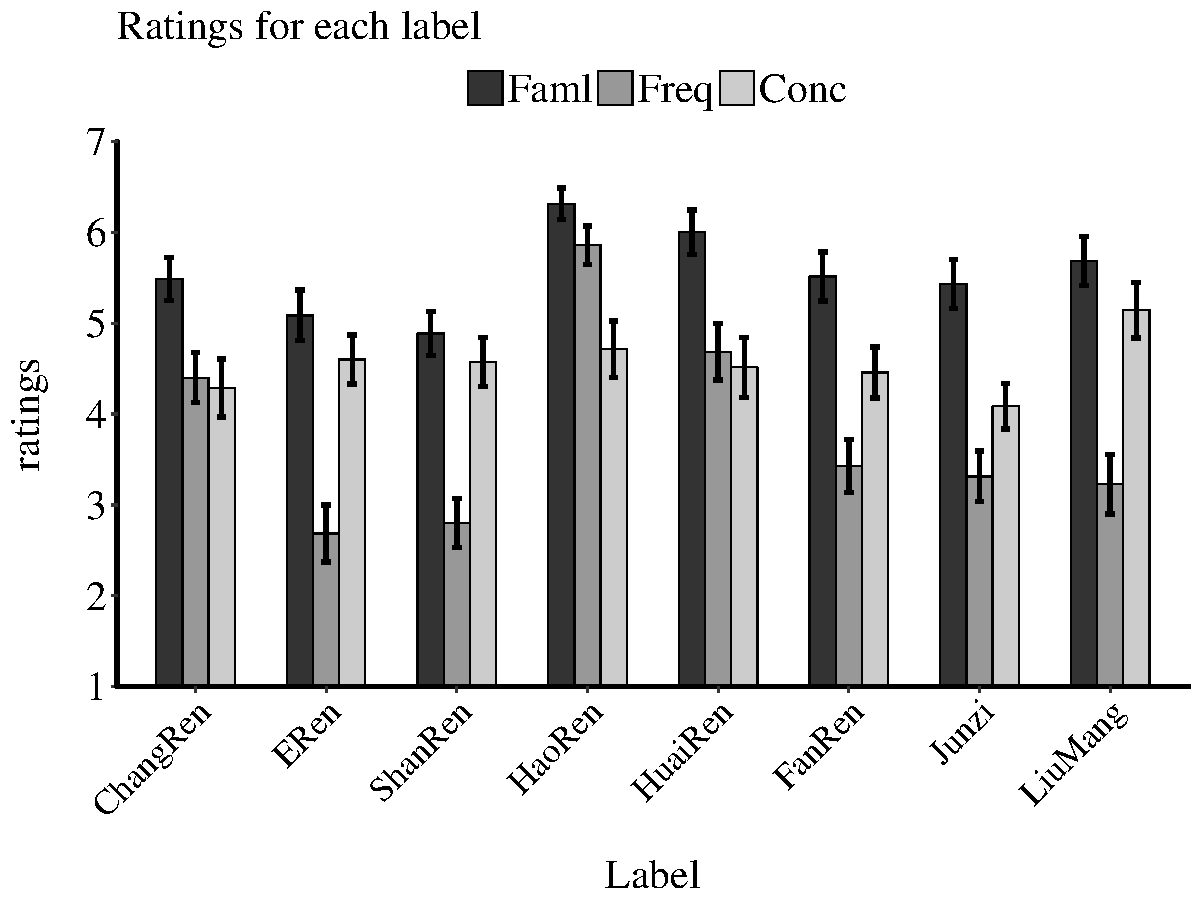
\includegraphics[width=5.20833in,height=\textheight]{exp1b/Familiarity_ratings/df1b_fami_rating.pdf}

\hypertarget{procedure-1}{%
\paragraph{Procedure}\label{procedure-1}}

For participants from both Tsinghua community and Wenzhou community, the procedure in the current study was exactly same as in experiment 1a.

\hypertarget{data-analysis-2}{%
\subsubsection{Data Analysis}\label{data-analysis-2}}

Data was analyzed as in experiment 1a.

\hypertarget{results-1}{%
\subsubsection{Results}\label{results-1}}

\hypertarget{nhst}{%
\paragraph{NHST}\label{nhst}}

Figure \ref{fig:ex1b-dprime-rt} shows \emph{d} prime and reaction times of experiment 1b.

\hypertarget{d-prime-1}{%
\subparagraph{d prime}\label{d-prime-1}}

Repeated measures ANOVA revealed main effect of valence, \(F(1.83, 93.20) = 14.98\), \(\mathit{MSE} = 0.18\), \(p < .001\), \(\hat{\eta}^2_G = .053\). Paired t test showed that the Good-Person condition (1.87 \(\pm\) 0.102) was with greater \emph{d} prime than Neutral condition (1.44 \(\pm\) 0.101, \emph{t}(51) = 5.945, \emph{p} \textless{} 0.001). We also found that the Bad-Person condition (1.67 \(\pm\) 0.11) has also greater \emph{d} prime than neutral condition , \emph{t}(51) = 3.132, \emph{p} = 0.008). There Good-person condition was also slightly greater than the bad condition, \emph{t}(51) = 2.265, \emph{p} = 0.0701.

\hypertarget{reaction-times-1}{%
\subparagraph{Reaction times}\label{reaction-times-1}}

We found interaction between Matchness and Valence (\(F(1.95, 99.31) = 19.71\), \(\mathit{MSE} = 960.92\), \(p < .001\), \(\hat{\eta}^2_G = .031\)) and then analyzed the matched trials and mismatched trials separately, as in experiment 1a. For matched trials, we found the effect of valence \(F(1.94, 99.10) = 33.97\), \(\mathit{MSE} = 1,343.19\), \(p < .001\), \(\hat{\eta}^2_G = .115\). Post-hoc \emph{t}-tests revealed that shapes associated with Good Person (684 \(\pm\) 8.77) were responded faster than Neutral-Person (740 \(\pm\) 9.84), (\emph{t}(51) = -8.167, \emph{p} \textless{} 0.001) and Bad Person (728 \(\pm\) 9.15), \emph{t}(51) = -5.724, \emph{p} \textless{} 0.0001). While there was no significant differences between Neutral and Bad-Person condition (\emph{t}(51) = 1.686, \emph{p} = 0.221). For non-matched trials, there was no significant effect of Valence (\(F(1.90, 97.13) = 1.80\), \(\mathit{MSE} = 430.15\), \(p = .173\), \(\hat{\eta}^2_G = .003\)).

\hypertarget{bglm}{%
\paragraph{BGLM}\label{bglm}}

\hypertarget{signal-detection-theory-analysis-of-accuracy}{%
\subparagraph{Signal detection theory analysis of accuracy}\label{signal-detection-theory-analysis-of-accuracy}}

We fitted a Bayesian hierarchical GLM for SDT. The results showed that when the shapes were tagged with labels with different moral valence, the sensitivity (\(d'\)) and criteria (\(c\)) were both influence. For the \(d'\), we found that the shapes tagged with morally good person (2.46, 95\% CI{[}2.21 2.72{]}) is greater than shapes tagged with moral bad (2.07, 95\% CI{[}1.83 2.32{]}), \(P_{PosteriorComparison} = 1\). Shape tagged with morally good person is also greater than shapes tagged with neutral person (2.23, 95\% CI{[}1.95 2.49{]}), \(P_{PosteriorComparison} = 0.97\). Also, the shapes tagged with neutral person is greater than shapes tagged with morally bad person, \(P_{PosteriorComparison} = 0.92\).

Interesting, we also found the criteria for three conditions also differ, the shapes tagged with good person has the highest criteria (-1.01, {[}-1.14 -0.88{]}), followed by shapes tagged with neutral person(1.06, {[}-1.21 -0.92{]}), and then the shapes tagged with bad person(-1.11, {[}-1.25 -0.97{]}). However, pair-wise comparison showed that only showed strong evidence for the difference between good and bad conditions.

\hypertarget{reaction-time}{%
\subparagraph{Reaction time}\label{reaction-time}}

We fitted a Bayesian hierarchical GLM for RTs, with a log-normal distribution as the link function. We used the posterior distribution of the regression coefficient to make statistical inferences. As in previous studies, the matched conditions are much faster than the mismatched trials (\(P_{PosteriorComparison} = 1\)). We focused on matched trials only, and compared different conditions: Good is faster than the neutral, \(P_{PosteriorComparison} = .99\), it was also faster than the Bad condition, \(P_{PosteriorComparison} = 1\). And the neutral condition is faster than the bad condition, \(P_{PosteriorComparison} = .99\). However, the mismatched trials are largely overlapped. See Figure \ref{fig:plot-exp1b-BGLM}.

\hypertarget{hddm-1}{%
\paragraph{HDDM}\label{hddm-1}}

We found that the shapes tagged with good person has higher drift rate and higher boundary separation than shapes tagged with both neutral and bad person. Also, the shapes tagged with neutral person has a higher drift rate than shapes tagged with bad person, but not for the boundary separation. Finally, we found that shapes tagged with bad person had longer non-decision time (see figure \ref{fig:plot-exp1b-HDDM}).

\hypertarget{discussion}{%
\subsubsection{Discussion}\label{discussion}}

These results confirmed the facilitation effect of positive moral valence on the perceptual matching task. This pattern of results mimic prior results demonstrating self-bias effect on perceptual matching (Sui et al., 2012) and in line with previous studies that indirect learning of other's moral reputation do have influence on our subsequent behavior (Fouragnan et al., 2013).

\hypertarget{experiment-1c}{%
\subsection{Experiment 1c}\label{experiment-1c}}

In this study, we further control the valence of words using in our experiment. Instead of using label with moral valence, we used valence-neutral names in China. Participant first learn behaviors of the different person, then, they associate the names and shapes. And then they perform a name-shape matching task.

\hypertarget{method-1}{%
\subsubsection{Method}\label{method-1}}

\hypertarget{participants-2}{%
\paragraph{Participants}\label{participants-2}}

23 college students (15 female, age = 22.61 \(\pm\) 2.62 years) participated. All of them were recruited from Tsinghua University community in 2014. Informed consent was obtained from all participants prior to the experiment according to procedures approved by the local ethics committees. No participant was excluded because they overall accuracy were above 0.6.

\hypertarget{stimuli-and-tasks-2}{%
\paragraph{Stimuli and Tasks}\label{stimuli-and-tasks-2}}

Three geometric shapes (triangle, square, and circle, with 3.7º × 3.7º of visual angle) were presented above a white fixation cross subtending 0.8º × 0.8º of visual angle at the center of the screen. The three most common names were chosen, which are neutral in moral valence before the manipulation.
Three names (Zhang, Wang, Li) were first paired with three paragraphs of behavioral description. Each description includes one sentence of biographic information and four sentences that describing the moral behavioral under that name. To assess the that these three descriptions represented good, neutral, and bad valence, we collected the ratings of three person on six dimensions: morality, likability, trustworthiness, dominance, competence, and aggressiveness, from an independent sample (n = 34, 18 female, age = 19.6 ± 2.05). The rating results showed that the person with morally good behavioral description has higher score on morality (M = 3.59, SD = 0.66) than neutral (M = 0.88, SD = 1.1), \emph{t}(33) = 12.94, \emph{p} \textless{} .001, and bad conditions (M = -3.4, SD = 1.1), \emph{t}(33) = 30.78, \emph{p} \textless{} .001. Neutral condition was also significant higher than bad conditions \(t(33) = 13.9\), \(p < .001\) (See supplementary materials).

\hypertarget{procedure-2}{%
\paragraph{Procedure}\label{procedure-2}}

After arriving the lab, participants were informed to complete two experimental tasks, first a social memory task to remember three person and their behaviors, after tested for their memory, they will finish a perceptual matching task.
In the social memory task, the descriptions of three person were presented without time limitation. Participant self-paced to memorized the behaviors of each person. After they memorizing, a recognition task was used to test their memory effect. Each participant was required to have over 95\% accuracy before preceding to matching task.
The perceptual learning task was followed, three names were randomly paired with geometric shapes. Participants were required to learn the association and perform a practicing task before they start the formal experimental blocks. They kept practicing until they reached 70\% accuracy. Then, they would start the perceptual matching task as in experiment 1a. They finished 6 blocks of perceptual matching trials, each have 120 trials.

\hypertarget{data-analysis-3}{%
\subsubsection{Data Analysis}\label{data-analysis-3}}

Data was analyzed as in experiment 1a.

\hypertarget{results-2}{%
\subsubsection{Results}\label{results-2}}

Figure \ref{fig:ex1c-dprime-rt} shows \emph{d} prime and reaction times of experiment 1c. We conducted same analysis as in Experiment 1a. Our analysis didn't should effect of valence on \emph{d} prime, \(F(1.93, 42.56) = 0.23\), \(\mathit{MSE} = 0.41\), \(p = .791\), \(\hat{\eta}^2_G = .005\). Neither the effect of valence on RT (\(F(1.63, 35.81) = 0.22\), \(\mathit{MSE} = 2,212.71\), \(p = .761\), \(\hat{\eta}^2_G = .001\)) or interaction between valence and matchness on RT (\(F(1.79, 39.43) = 1.20\), \(\mathit{MSE} = 1,973.91\), \(p = .308\), \(\hat{\eta}^2_G = .005\)).

\hypertarget{signal-detection-theory-analysis-of-accuracy-1}{%
\paragraph{Signal detection theory analysis of accuracy}\label{signal-detection-theory-analysis-of-accuracy-1}}

We fitted a Bayesian hierarchical GLM for SDT. The results showed that when the shapes were tagged with labels with different moral valence, the sensitivity (\(d'\)) and criteria (\(c\)) were both influenced. For the \(d'\), we found that the shapes tagged with morally good person (2.30, 95\% CI{[}1.93 2.70{]}) is greater than shapes tagged with moral bad (2.11, 95\% CI{[}1.83 2.42{]}), \(P_{PosteriorComparison} = 0.8\). Shape tagged with morally good person is also greater than shapes tagged with neutral person (2.16, 95\% CI{[}1.88 2.45{]}), \(P_{PosteriorComparison} = 0.75\).

Interesting, we also found the criteria for three conditions also differ, the shapes tagged with good person has the highest criteria (-0.97, {[}-1.12 -0.82{]}), followed by shapes tagged with neutral person(-0.96, {[}-1.09 -0.83{]}), and then the shapes tagged with bad person(-1.03, {[}-1.22 -0.84{]}). However, pair-wise comparison showed that only showed strong evidence for the difference between good and bad conditions.

\hypertarget{reaction-time-1}{%
\paragraph{Reaction time}\label{reaction-time-1}}

We fitted a Bayesian hierarchical GLM for RTs, with a log-normal distribution as the link function. We used the posterior distribution of the regression coefficient to make statistical inferences. As in previous studies, the matched conditions are much faster than the mismatched trials (\(P_{PosteriorComparison} = .75\)). We focused on matched trials only, and compared different conditions: Good () is not faster than the neutral (), \(P_{PosteriorComparison} = .5\), it was faster than the Bad condition (), \(P_{PosteriorComparison} = .88\). And the neutral condition is faster than the bad condition, \(P_{PosteriorComparison} = .95\). However, the mismatched trials are largely overlapped.

\hypertarget{hddm-2}{%
\subsubsection{HDDM}\label{hddm-2}}

We fitted our data with HDDM, using the response-coding (also see Hu et al., 2020). We estimated separate drift rate (\(v\)), non-decision time (\(T_{0}\)), and boundary separation (\(a\)) for each condition. We found that the shapes tagged with good person has higher drift rate and higher boundary separation than shapes tagged with both neutral and bad person. Also, the shapes tagged with neutral person has a higher drift rate than shapes tagged with bad person, but not for the boundary separation. Finally, we found that shapes tagged with bad person had longer non-decision time (see figure \ref{fig:plot-exp1c-HDDM})).

\hypertarget{experiment-2-sequential-presenting}{%
\subsection{Experiment 2: Sequential presenting}\label{experiment-2-sequential-presenting}}

Experiment 2 was conducted for two purpose: (1) to further confirm the facilitation effect of positive moral associations; (2) to test the effect of expectation of occurrence of each pair. In this experiment, after participant learned the association between labels and shapes, they were presented a label first and then a shape, they then asked to judge whether the shape matched the label or not (see (Sui, Sun, Peng, \& Humphreys, 2014). Previous studies showed that when the labels presented before the shapes, participants formed expectations about the shape, and therefore a top-down process were introduced into the perceptual matching processing. If the facilitation effect of positive moral valence we found in experiment 1 was mainly drive by top-down processes, this sequential presenting paradigm may eliminate or attenuate this effect; if, however, the facilitation effect occurred because of button-up processes, then, similar facilitation effect will appear even with sequential presenting paradigm.

\hypertarget{method-2}{%
\subsubsection{Method}\label{method-2}}

\hypertarget{participants-3}{%
\paragraph{Participants}\label{participants-3}}

35 participants (17 female, age = 21.66 \(\pm\) 3.03) were recruited. 24 of them had participated in Experiment 1a (9 male, mean age = 21.9, s.d. = 2.9), and the time gap between these experiment 1a and experiment 2 is at least six weeks. The results of 1 participants were excluded from analysis because of less than 60\% overall accuracy, remains 34 participants (17 female, age = 21.74 \(\pm\) 3.04).

\hypertarget{procedure-3}{%
\paragraph{Procedure}\label{procedure-3}}

In Experiment 2, the sequential presenting makes the matching task much easier than experiment 1. To avoid ceiling effect on behavioral data, we did a few pilot experiments to get optimal parameters, i.e., the conditions under which participant have similar accuracy as in Experiment 1 (around 70 \textasciitilde{} 80\% accuracy).
In the final procedure, the label (good person, bad person, or neutral person) was presented for 50 ms and then masked by a scrambled image for 200 ms. A geometric shape followed the scrambled mask for 50 ms in a noisy background (which was produced by first decomposing a square with \(¾\) gray area and \(¼\) white area to small squares with a size of 2 × 2 pixels and then re-combine these small pieces randomly), instead of pure gray background in Experiment 1. After that, a blank screen was presented 1100 ms, during which participants should press a button to indicate the label and the shape match the original association or not. Feedback was given, as in study 1. The next trial then started after 700 \textasciitilde{} 1100 ms blank. Other aspects of study 2 were identical to study 1.

\hypertarget{data-analysis-4}{%
\paragraph{Data analysis}\label{data-analysis-4}}

Data was analyzed as in study 1a.

\hypertarget{results-3}{%
\subsubsection{Results}\label{results-3}}

\hypertarget{nhst-1}{%
\paragraph{NHST}\label{nhst-1}}

Figure \ref{fig:ex2-dprime-rt} shows \emph{d} prime and reaction times of experiment 2. Less than 0.2\% correct trials with less than 200ms reaction times were excluded.

\hypertarget{d-prime.}{%
\subparagraph{d prime.}\label{d-prime.}}

There was evidence for the main effect of valence, \(F(1.83, 60.36) = 14.41\), \(\mathit{MSE} = 0.23\), \(p < .001\), \(\hat{\eta}^2_G = .066\). Paired t test showed that the Good-Person condition (2.79 \(\pm\) 0.17) was with greater \emph{d} prime than Netural condition (2.21 \(\pm\) 0.16, \emph{t}(33) = 4.723, \emph{p} = 0.001) and Bad-person condition (2.41 \(\pm\) 0.14), \emph{t}(33) = 4.067, \emph{p} = 0.008). There was no-significant difference between Neutral-person and Bad-person conidition, \emph{t}(33) = -1,802, \emph{p} = 0.185.

\hypertarget{reaction-time-2}{%
\subparagraph{Reaction time}\label{reaction-time-2}}

The results of reaction times of matchness trials showed similar pattern as the \emph{d} prime data.

We found interaction between Matchness and Valence (\(F(1.99, 65.70) = 9.53\), \(\mathit{MSE} = 605.36\), \(p < .001\), \(\hat{\eta}^2_G = .017\)) and then analyzed the matched trials and mismatched trials separately, as in experiment 1a. For matched trials, we found the effect of valence \(F(1.99, 65.76) = 10.57\), \(\mathit{MSE} = 1,192.65\), \(p < .001\), \(\hat{\eta}^2_G = .067\). Post-hoc \emph{t}-tests revealed that shapes associated with Good Person (548 \(\pm\) 9.4) were responded faster than Neutral-Person (582 \(\pm\) 10.9), (\emph{t}(33) = -3.95, \emph{p} = 0.0011) and Bad Person (582 \(\pm\) 10.2), \emph{t}(33) = -3.9, \emph{p} = 0.0013). While there was no significant differences between Neutral and Bad-Person condition (\emph{t}(33) = -0.01, \emph{p} = 0.999). For non-matched trials, there was no significant effect of Valence (\(F(1.99, 65.83) = 0.17\), \(\mathit{MSE} = 489.80\), \(p = .843\), \(\hat{\eta}^2_G = .001\)).

\hypertarget{bglmm}{%
\paragraph{BGLMM}\label{bglmm}}

\hypertarget{signal-detection-theory-analysis-of-accuracy-2}{%
\subparagraph{Signal detection theory analysis of accuracy}\label{signal-detection-theory-analysis-of-accuracy-2}}

We fitted a Bayesian hierarchical GLM for SDT. The results showed that when the shapes were tagged with labels with different moral valence, the sensitivity (\(d'\)) and criteria (\(c\)) were both influence. For the \(d'\), we found that the shapes tagged with morally good person (2.46, 95\% CI{[}2.21 2.72{]}) is greater than shapes tagged with moral bad (2.07, 95\% CI{[}1.83 2.32{]}), \(P_{PosteriorComparison} = 1\). Shape tagged with morally good person is also greater than shapes tagged with neutral person (2.23, 95\% CI{[}1.95 2.49{]}), \(P_{PosteriorComparison} = 0.97\). Also, the shapes tagged with neutral person is greater than shapes tagged with morally bad person, \(P_{PosteriorComparison} = 0.92\).

Interesting, we also found the criteria for three conditions also differ, the shapes tagged with good person has the highest criteria (-1.01, {[}-1.14 -0.88{]}), followed by shapes tagged with neutral person(1.06, {[}-1.21 -0.92{]}), and then the shapes tagged with bad person(-1.11, {[}-1.25 -0.97{]}). However, pair-wise comparison showed that only showed strong evidence for the difference between good and bad conditions.

\hypertarget{reaction-times-2}{%
\subparagraph{Reaction times}\label{reaction-times-2}}

We fitted a Bayesian hierarchical GLM for RTs, with a log-normal distribution as the link function. We used the posterior distribution of the regression coefficient to make statistical inferences. As in previous studies, the matched conditions are much faster than the mismatched trials (\(P_{PosteriorComparison} = .75\)). We focused on matched trials only, and compared different conditions: Good () is not faster than the neutral (), \(P_{PosteriorComparison} = .5\), it was faster than the Bad condition (), \(P_{PosteriorComparison} = .88\). And the neutral condition is faster than the bad condition, \(P_{PosteriorComparison} = .95\). However, the mismatched trials are largely overlapped.

\hypertarget{hddm-3}{%
\subsubsection{HDDM}\label{hddm-3}}

We fitted our data with HDDM, using the response-coding (also see Hu et al., 2020). We estimated separate drift rate (\(v\)), non-decision time (\(T_{0}\)), and boundary separation (\(a\)) for each condition. We found that the shapes tagged with good person has higher drift rate and higher boundary separation than shapes tagged with both neutral and bad person. Also, the shapes tagged with neutral person has a higher drift rate than shapes tagged with bad person, but not for the boundary separation. Finally, we found that shapes tagged with bad person had longer non-decision time (see figure @ref(fig:plot-exp1c
-HDDM))).

\hypertarget{discussion-1}{%
\subsection{Discussion}\label{discussion-1}}

In this experiment, we repeated the results pattern that the positive moral valenced stimuli has an advantage over the neutral or the negative valence association. Moreover, with a cross-task analysis, we did not find evidence that the experiment task interacted with moral valence, suggesting that the effect might not be effect by experiment task.
These findings suggested that the facilitation effect of positive moral valence is robust and not affected by task. This robust effect detected by the associative learning is unexpected.

\hypertarget{experiment-6a-eeg-study-1}{%
\subsection{Experiment 6a: EEG study 1}\label{experiment-6a-eeg-study-1}}

Experiment 6a was conducted to study the neural correlates of the positive prioritization effect. The behavioral paradigm is same as experiment 2.

\hypertarget{method-3}{%
\subsubsection{Method}\label{method-3}}

\hypertarget{participants-4}{%
\paragraph{Participants}\label{participants-4}}

24 college students (8 female, age = 22.88 \(\pm\) 2.79) participated the current study, all of them were from Tsinghua University in 2014. Informed consent was obtained from all participants prior to the experiment according to procedures approved by a local ethics committee. No participant was excluded from behavioral analysis.

\hypertarget{experimental-design}{%
\subsubsection{Experimental design}\label{experimental-design}}

The experimental design of this experiment is same as experiment 2: a 3 × 2 within-subject design with moral valence (good, neutral and bad associations) and matchness between shape and label (match vs.~mismatch for the personal association) as within-subject variables.

\hypertarget{stimuli}{%
\paragraph{Stimuli}\label{stimuli}}

Three geometric shapes (triangle, square and circle, each 4.6º × 4.6º of visual angle) were presented at the center of screen for 50 ms after 500ms of fixation (0.8º × 0.8º of visual angle). The association of the three shapes to bad person (\enquote{坏人, HuaiRen}), good person (\enquote{好人, HaoRen}) or ordinary person (\enquote{常人, ChangRen}) was counterbalanced across participants. The words bad person, good person or ordinary person (3.6º × 1.6º) was also displayed at the center fo the screen. Participants had to judge whether the pairings of label and shape matched (e.g., Does the circle represent a bad person?). The experiment was run on a PC using E-prime software (version 2.0). These stimuli were displayed on a 22-in CRT monitor (1024×768 at 100Hz).
We used backward masking to avoid over-processing of the moral words, in which a scrambled picture were presented for 900 ms after the label. Also, to avoid the ceiling effect on accuracy, shapes were presented on a noisy background based on our pilot studies. The noisy images were made by scrambling a picture of 3/4gray and ¼ white at resolution of 2 × 2 pixel.

\hypertarget{procedure-4}{%
\paragraph{Procedure}\label{procedure-4}}

The procedure was similar to Experiment 2. Participants finished 9 blocks of trial, each with 120 trials. In total, participants finished 180 trials for each combination of condition.

As in experiment 2 (Sui, He, \& Humphreys, 2012), subjects first learned the associations between labels and shapes and then completed a shape-label matching task (e.g., good person-triangle). In each trial of the matching task, a fixation were first presented for 500 ms, followed by a 50 ms label; then, a scrambled picture presented 900 ms. After the backward mask, the shape were presented on a noisy background for 50ms. Participant have to response in 1000ms after the presentation of the shape, and finally, a feedback screen was presented for 500 ms (see figure 1). The inter-trial interval (ITI) were randomly varied at the range of 1000 \textasciitilde{} 1400 ms.

All the stimuli were presented on a gray background (RGB: 127, 127, 127). E-primed 2.0 was used to present stimuli and collect behavioral results. Data were collected and analyzed when accuracy performance in total reached 60\%.

\hypertarget{data-analysis-5}{%
\subsubsection{Data Analysis}\label{data-analysis-5}}

Data was analyzed as in experiment 1a.

\hypertarget{results-4}{%
\subsubsection{Results}\label{results-4}}

\hypertarget{nhst-2}{%
\paragraph{NHST}\label{nhst-2}}

Only the behavioral results were reported here. Figure \ref{fig:ex6a-dprime-rt} shows \emph{d} prime and reaction times of experiment 6a.

\hypertarget{d-prime-2}{%
\subparagraph{d prime}\label{d-prime-2}}

We conducted repeated measures ANOVA, with moral valence as independent variable. The results revealed the main effect of valence (\(F(1.74, 40.05) = 3.76\), \(\mathit{MSE} = 0.10\), \(p = .037\), \(\hat{\eta}^2_G = .021\)). Post-hoc analysis revealed that shapes link with Good person (mean = 3.13, SE = 0.109) is greater than Neutral condition (mean = 2.88, SE = 0.14),\emph{t} = 2.916, \emph{df} = 24, \emph{p} = 0.02, p-value adjusted by Tukey method, but the \emph{d} prime between Good and bad (mean = 3.03, SE = 0.142) (\emph{t} = 1.512, \emph{df} = 24, \emph{p} = 0.3034, p-value adjusted by Tukey method), bad and neutral (\emph{t} = 1.599, \emph{df} = 24, \emph{p} = 0.2655, p-value adjusted by Tukey method) were not significant.

\hypertarget{reaction-times.}{%
\subparagraph{Reaction times.}\label{reaction-times.}}

The results of reaction times of matchness trials showed similar pattern as the \emph{d} prime data.

We found intercation between Matchness and Valence (\(F(1.97, 45.20) = 20.45\), \(\mathit{MSE} = 450.47\), \(p < .001\), \(\hat{\eta}^2_G = .021\)) and then analyzed the matched trials and mismatched trials separately, as in experiment 2. For matched trials, we found the effect of valence \(F(1.97, 45.25) = 32.37\), \(\mathit{MSE} = 522.42\), \(p < .001\), \(\hat{\eta}^2_G = .078\). For non-matched trials, there was no significant effect of Valence (\(F(1.77, 40.67) = 0.35\), \(\mathit{MSE} = 242.15\), \(p = .679\), \(\hat{\eta}^2_G = .000\)). Post-hoc \emph{t}-tests revealed that shapes associated with Good Person (mean = 550, SE = 13.8) were responded faster than Neutral-Person (501, SE = 14.7), (\emph{t}(24) = -5.171, \emph{p} = 0.0001) and Bad Person (523, SE = 16.3), \emph{t}(24) = -8.137, \emph{p} \textless{} 0.0001)., and Neutral is faster than Bad-Person condition (\emph{t}(32) = -3.282, \emph{p} = 0.0085).

\hypertarget{bglm-1}{%
\paragraph{BGLM}\label{bglm-1}}

\hypertarget{signal-detection-theory-analysis-of-accuracy-3}{%
\subparagraph{Signal detection theory analysis of accuracy}\label{signal-detection-theory-analysis-of-accuracy-3}}

\hypertarget{reaction-time-3}{%
\subparagraph{Reaction time}\label{reaction-time-3}}

\hypertarget{hddm-4}{%
\subsubsection{HDDM}\label{hddm-4}}

We fitted our data with HDDM, using the response-coding (also see Hu et al., 2020). We estimated separate drift rate (\(v\)), non-decision time (\(T_{0}\)), and boundary separation (\(a\)) for each condition. We found that, similar to experiment 2, the shapes tagged with good person has higher drift rate and higher boundary separation than shapes tagged with both neutral and bad person, but only for the self-referential condition. Also, the shapes tagged with neutral person has a higher drift rate than shapes tagged with bad person, but not for the boundary separation, and this effect also exist only for the self-referential condition.

Interestingly, we found that in both self-referential and other-referential conditions, the shapes associated bad valence have higher drift rate and higher boundary separation. which might suggest that the shape associated with bad stimuli might be prioritized in the non-match trials (see figure \ref{fig:plot-exp6a-HDDM}).

\begin{sidewaysfigure}
\includegraphics{Notebook_Pos_Self_Salience_APA_files/figure-latex/unnamed-chunk-7-1} \caption{Results for part 1.}\label{fig:unnamed-chunk-7}
\end{sidewaysfigure}

\hypertarget{part-2-interaction-between-valence-and-identity}{%
\section{Part 2: interaction between valence and identity}\label{part-2-interaction-between-valence-and-identity}}

In this part, we report two experiments that aimed at testing whether the moral valence effect found in the previous experiment can be modulated by the self-referential processing.

\hypertarget{experiment-3a}{%
\subsection{Experiment 3a}\label{experiment-3a}}

To examine the modulation effect of positive valence was an intrinsic, self-referential process, we designed study 3. In this study, moral valence was assigned to both self and a stranger. We hypothesized that the modulation effect of moral valence will be stronger for the self than for a stranger.

\hypertarget{method-4}{%
\subsubsection{Method}\label{method-4}}

\hypertarget{participants-5}{%
\paragraph{Participants}\label{participants-5}}

38 college students (15 female, age = 21.92 \(\pm\) 2.16) participated in experiment 3a. All of them were right-handed, and all had normal or corrected-to-normal vision. Informed consent was obtained from all participants prior to the experiment according to procedures approved by a local ethics committee. One female and one male student did not finish the experiment, and 1 participants' data were excluded from analysis because less than 60\% overall accuracy, remains 35 participants (13 female, age = 22.11 \(\pm\) 2.13).

\hypertarget{design}{%
\paragraph{Design}\label{design}}

Study 3a combined moral valence with self-relevance, hence the experiment has a 2 × 3 × 2 within-subject design. The first variable was self-relevance, include two levels: self-relevance vs.~stranger-relevance; the second variable was moral valence, include good, neutral and bad; the third variable was the matching between shape and label: match vs.~nonmatch.

\hypertarget{stimuli-1}{%
\paragraph{Stimuli}\label{stimuli-1}}

The stimuli used in study 3a share the same parameters with experiment 1 \& 2. The differences was that we used six shapes: triangle, square, circle, trapezoid, diamond, regular pentagon, and six labels: good self, neutral self, bad self, good person, bad person, and neutral person. To match the concreteness of the label, we asked participant to chosen an unfamiliar name of their own gender to be the stranger.

\hypertarget{procedure-5}{%
\paragraph{Procedure}\label{procedure-5}}

After being fully explained and signed the informed consent, participants were instructed to chose a name that can represent a stranger with same gender as the participant themselves, from a common Chinese name pool. Before experiment, the experimenter explained the meaning of each label to participants. For example, the \enquote{good self} mean the morally good side of themselves, them could imagine the moment when they do something's morally applauded, \enquote{bad self} means the morally bad side of themselves, they could also imagine the moment when they doing something morally wrong, and \enquote{neutral self} means the aspect of self that does not related to morality, they could imagine the moment when they doing something irrelevant to morality. In the same sense, the \enquote{good other}, \enquote{bad other}, and \enquote{neutral other} means the three different aspects of the stranger, whose name was chosen before the experiment. Then, the experiment proceeded as study 1a. Each participant finished 6 blocks, each have 120 trials. The sequence of trials was pseudo-randomized so that there are 10 matched trials for each condition and 10 non-matched trials for each condition (good self, neutral self, bad self, good other, neutral other, bad other) for each block.

\hypertarget{data-analysis-6}{%
\paragraph{Data Analysis}\label{data-analysis-6}}

Data analysis followed strategies described in the general method section. Reaction times and \emph{d} prime data were analyzed as in study 1 and study 2, except that one more within-subject variable (i.e., self-relevance) was included in the analysis.

\hypertarget{results-5}{%
\subsubsection{Results}\label{results-5}}

\hypertarget{nhst-3}{%
\paragraph{NHST}\label{nhst-3}}

\begin{figure}
\centering
\includegraphics{Notebook_Pos_Self_Salience_APA_files/figure-latex/ex3a-dprime-rt-1.pdf}
\caption{\label{fig:ex3a-dprime-rt}RT and \emph{d} prime of Experiment 3a.}
\end{figure}

Figure \ref{fig:ex3a-dprime-rt} shows \emph{d} prime and reaction times of experiment 3a. Less than 5\% correct trials with less than 200ms reaction times were excluded.

\hypertarget{d-prime-3}{%
\subparagraph{d prime}\label{d-prime-3}}

There was evidence for the main effect of valence, \(F(1.89, 64.37) = 11.09\), \(\mathit{MSE} = 0.23\), \(p < .001\), \(\hat{\eta}^2_G = .039\), and main effect of self-relevance, \(F(1, 34) = 3.22\), \(\mathit{MSE} = 0.54\), \(p = .082\), \(\hat{\eta}^2_G = .015\), as well as the interaction, \(F(1.79, 60.79) = 3.39\), \(\mathit{MSE} = 0.43\), \(p = .045\), \(\hat{\eta}^2_G = .022\).

We then conducted separated ANOVA for self-referential and other-referential trials. The valence effect was shown for the self-referential conditions, \(F(1.65, 56.25) = 13.98\), \(\mathit{MSE} = 0.31\), \(p < .001\), \(\hat{\eta}^2_G = .119\). Post-hoc test revealed that the Good-Self condition (1.97 \(\pm\) 0.14) was with greater \emph{d} prime than Netural condition (1.41 \(\pm\) 0.12, \emph{t}(34) = 4.505, \emph{p} = 0.0002), and Bad-self condition (1.43 \(\pm\) 0.102), \emph{t}(34) = 3.856, \emph{p} = 0.0014. There was difference between neutral and bad condition, \emph{t}(34) = -0.238, \emph{p} = 0.9694. However, no effect of valence was found for the other-referential condition \(F(1.98, 67.36) = 0.38\), \(\mathit{MSE} = 0.35\), \(p = .681\), \(\hat{\eta}^2_G = .004\).

\hypertarget{reaction-time-4}{%
\subparagraph{Reaction time}\label{reaction-time-4}}

We found interaction between Matchness and Valence (\(F(1.98, 67.44) = 26.29\), \(\mathit{MSE} = 730.09\), \(p < .001\), \(\hat{\eta}^2_G = .025\)) and then analyzed the matched trials and nonmatch trials separately, as in previous experiments.

For the match trials, we found that the interaction between identity and valence, \(F(1.72, 58.61) = 3.89\), \(\mathit{MSE} = 2,750.19\), \(p = .032\), \(\hat{\eta}^2_G = .019\), as well as the main effect of valence \(F(1.98, 67.34) = 35.76\), \(\mathit{MSE} = 1,127.25\), \(p < .001\), \(\hat{\eta}^2_G = .079\), but not the effect of identity \(F(1, 34) = 0.20\), \(\mathit{MSE} = 3,507.14\), \(p = .660\), \(\hat{\eta}^2_G = .001\). As for the \emph{d} prime, we separated analyzed the self-referential and other-referential trials. For the Self-referential trials, we found the main effect of valence, \(F(1.80, 61.09) = 30.39\), \(\mathit{MSE} = 1,584.53\), \(p < .001\), \(\hat{\eta}^2_G = .159\); for the other-referential trials, the effect of valence is weaker, \(F(1.86, 63.08) = 2.85\), \(\mathit{MSE} = 2,224.30\), \(p = .069\), \(\hat{\eta}^2_G = .024\). We then focused on the self conditions: the good-self condition (713 \(\pm\) 12) is faster than neutral- (776 \(\pm\) 11.8), \emph{t}(34) = -7.396, \emph{p} \textless{} .0001 , and bad-self (772 \(\pm\) 10.1) conditions, \emph{t}(34) = -5.66, \emph{p} \textless{} .0001. But there is not difference between neutral- and bad-self conditions, \emph{t}(34) = 0.481, \emph{p} = 0.881.

For the nonmatch trials, we didn't found any strong effect: identity, \(F(1, 34) = 3.43\), \(\mathit{MSE} = 660.02\), \(p = .073\), \(\hat{\eta}^2_G = .004\), valence \(F(1.89, 64.33) = 0.40\), \(\mathit{MSE} = 444.10\), \(p = .661\), \(\hat{\eta}^2_G = .001\), or interaction between the two \(F(1.94, 66.02) = 2.42\), \(\mathit{MSE} = 817.35\), \(p = .099\), \(\hat{\eta}^2_G = .007\).

\hypertarget{bglm-2}{%
\paragraph{BGLM}\label{bglm-2}}

\hypertarget{signal-detection-theory-analysis-of-accuracy-4}{%
\subparagraph{Signal detection theory analysis of accuracy}\label{signal-detection-theory-analysis-of-accuracy-4}}

We found that the \emph{d} prime is greater when shapes were associated with good self condition than with neutral self or bad self, but shapes associated with bad self and neutral self didn't show differences. Comparing the self vs other under three condition revealed that shapes associated with good self is greater than with good other, but with a weak evidence. In contrast, for both neutral and bad valence condition, shapes associated with other had greater \emph{d} prime than with self.

\hypertarget{reaction-time-5}{%
\subparagraph{Reaction time}\label{reaction-time-5}}

\begin{figure}
\centering
\includegraphics{Notebook_Pos_Self_Salience_APA_files/figure-latex/plot-exp3a-BGLM-1.pdf}
\caption{\label{fig:plot-exp3a-BGLM}Exp3a: Results of Bayesian GLM analysis.}
\end{figure}

In reaction times, we found that same trends in the match trials as in the RT: while the shapes associated with good self was greater than with good other (log mean diff = -0.02858, 95\%HPD{[}-0.070898, 0.0154{]}), the direction is reversed for neutral and negative condition. see Figure \ref{fig:plot-exp3a-BGLM}

\hypertarget{hddm-5}{%
\subsubsection{HDDM}\label{hddm-5}}

\begin{figure}
\centering
\includegraphics{Notebook_Pos_Self_Salience_APA_files/figure-latex/plot-exp3a-HDDM-1.pdf}
\caption{\label{fig:plot-exp3a-HDDM}Exp3a: Results of HDDM.}
\end{figure}

We fitted our data with HDDM, using the response-coding (also see Hu et al., 2020). We estimated separate drift rate (\(v\)), non-decision time (\(T_{0}\)), and boundary separation (\(a\)) for each condition. We found that the shapes tagged with good person has higher drift rate and higher boundary separation than shapes tagged with both neutral and bad person. Also, the shapes tagged with neutral person has a higher drift rate than shapes tagged with bad person, but not for the boundary separation. Finally, we found that shapes tagged with bad person had longer non-decision time (see figure \ref{fig:plot-exp3a-HDDM})).

\hypertarget{experiment-3b}{%
\subsection{Experiment 3b}\label{experiment-3b}}

In study 3a, participants had to remember 6 pairs of association, which cause high cognitive load during the whole experiment. To eliminate the influence of cognitive load, we conducted study 3b, in which participant learn three aspect of self and stranger separately in to consecutive task. We hypothesize that we will replicate the pattern of study 3a, i.e., the effect of moral valence only occurs for self-relevant conditions.
\#\#\# Method

\hypertarget{participants-6}{%
\paragraph{Participants}\label{participants-6}}

Study 3b were finished in 2017, at that time we have calculated that the effect size (Cohen's \(d\)) of good-person (or good-self) vs.~bad-person (or bad-other) was between 0.47 \textasciitilde{} 0.53, based on the data from Tsinghua community in study 1a, 1b, 2, 3a, 4a, and 4b. Based on this effect size, we estimated that 54 participants would allow we to detect the effect size of Cohen's = 0.5 with 95\% power and alpha = 0.05, using G*power 3.192 (Faul, Erdfelder, Buchner, \& Lang, 2009). Therefore, we planned to stop after we arrived this number. During the data collected at Wenzhou University, 61 participants (45 females; 19 to 25 years of age, age = 20.42 \(\pm\) 1.77) came to the testing room and we tested all of them during a single day. All participants were right-handed, and all had normal or corrected-to-normal vision. Informed consent was obtained from all participants prior to the experiment according to procedures approved by a local ethics committee. 4 participants' data were excluded from analysis because their over all accuracy was lower than 60\%, 1 more participant was excluded because of zero hit rate for one condition, leaving 56 participants (43 females; 19 to 25 years old, age = 20.27 \(\pm\) 1.60).

\hypertarget{design-1}{%
\paragraph{Design}\label{design-1}}

Study 3b has the same experimental design as 3a, with a 2× 3× 2 within-subject design. The first variable was self-relevance, include two levels: self-relevant vs.~stranger-relevant; the second variable was moral valence, include good, neutral and bad; the third variable was the matching between shape and label: match vs.~mismatch.
Stimuli. The stimuli used in study 3b share the same parameters with experiment 3a. 6 shapes were included (triangle, square, circle, trapezoid, diamond, regular pentagon), as well as 6 labels, but the labels changed to \enquote{good self}, \enquote{neutral self}, \enquote{bad self}, \enquote{good him/her}, bad him/her'', \enquote{neutral him/her}, the stranger's label is consistent with participants' gender. Same as study 3a, we asked participant to chosen an unfamiliar name of their own gender to be the stranger before showing them the relationship. Note, because of implementing error, the personal distance data did not collect for this experiment.

\hypertarget{stimuli-2}{%
\paragraph{Stimuli}\label{stimuli-2}}

The stimuli used in study 3b is the same as in experiment 3a.

\hypertarget{procedure-6}{%
\paragraph{Procedure}\label{procedure-6}}

In this experiment, participants finished two matching tasks, i.e., self-matching task, and other-matching task. In the self-matching task, participants first associate the three aspects of self to three different shapes, and then perform the matching task. In the other-matching task, participants first associate the three aspects of the stranger to three different shapes, and then perform the matching task. The order of self-task and other-task are counter-balanced among participants.
Different from experiment 3a, after presenting the stimuli pair for 100ms, participant has 1900 ms to response, and they feedback with both accuracy and reaction time.
As in study 3a, before each task, the instruction showed the meaning of each label to participants. The self-matching task and other-matching task were randomized between participants. Each participant finished 6 blocks, each have 120 trials.

\hypertarget{data-analysis-7}{%
\paragraph{Data Analysis}\label{data-analysis-7}}

Same as experiment 3a.

\hypertarget{results-6}{%
\subsubsection{Results}\label{results-6}}

\hypertarget{nhst-4}{%
\paragraph{NHST}\label{nhst-4}}

\begin{figure}
\centering
\includegraphics{Notebook_Pos_Self_Salience_APA_files/figure-latex/exp3b-dprime-rt-1.pdf}
\caption{\label{fig:exp3b-dprime-rt}RT and \emph{d} prime of Experiment 3b.}
\end{figure}

Figure \ref{fig:exp3b-dprime-rt} shows \emph{d} prime and reaction times of experiment 3b. Less than 5\% correct trials with less than 200ms reaction times were excluded.

\hypertarget{d-prime-4}{%
\subparagraph{d prime}\label{d-prime-4}}

There was no evidence for the main effect of valence, \(F(1.92, 105.43) = 1.90\), \(\mathit{MSE} = 0.33\), \(p = .157\), \(\hat{\eta}^2_G = .005\), but we found a main effect of self-relevance, \(F(1, 55) = 4.65\), \(\mathit{MSE} = 0.89\), \(p = .035\), \(\hat{\eta}^2_G = .017\), as well as the interaction, \(F(1.90, 104.36) = 5.58\), \(\mathit{MSE} = 0.26\), \(p = .006\), \(\hat{\eta}^2_G = .011\).

We then conducted separated ANOVA for self-referential and other-referential trials. The valence effect was shown for the self-referential conditions, \(F(1.75, 96.42) = 6.73\), \(\mathit{MSE} = 0.30\), \(p = .003\), \(\hat{\eta}^2_G = .037\). Post-hoc test revealed that the Good-Self condition (2.15 \(\pm\) 0.12) was with greater \emph{d} prime than Neutral condition (1.83 \(\pm\) 0.12, \emph{t}(34) = 3.36, \emph{p} = 0.0031), and Bad-self condition (1.87 \(\pm\) 0.12), \emph{t}(34) = 2.955, \emph{p} = 0.01. There was difference between neutral and bad condition, \emph{t}(34) = -0.039, \emph{p} = 0.914. However, no effect of valence was found for the other-referential condition \(F(1.93, 105.97) = 0.61\), \(\mathit{MSE} = 0.31\), \(p = .539\), \(\hat{\eta}^2_G = .002\).

\hypertarget{reaction-time-6}{%
\subparagraph{Reaction time}\label{reaction-time-6}}

We found interaction between Matchness and Valence (\(F(1.86, 102.47) = 15.44\), \(\mathit{MSE} = 3,112.78\), \(p < .001\), \(\hat{\eta}^2_G = .006\)) and then analyzed the matched trials and nonmatch trials separately, as in previous experiments.

For the match trials, we found that the interaction between identity and valence, \(F(1.67, 92.11) = 6.14\), \(\mathit{MSE} = 6,472.48\), \(p = .005\), \(\hat{\eta}^2_G = .009\), as well as the main effect of valence \(F(1.88, 103.65) = 24.25\), \(\mathit{MSE} = 5,994.25\), \(p < .001\), \(\hat{\eta}^2_G = .038\), but not the effect of identity \(F(1, 55) = 48.49\), \(\mathit{MSE} = 25,892.59\), \(p < .001\), \(\hat{\eta}^2_G = .153\). As for the \emph{d} prime, we separated analyzed the self-referential and other-referential trials. For the Self-referential trials, we found the main effect of valence, \(F(1.66, 91.38) = 23.98\), \(\mathit{MSE} = 6,965.61\), \(p < .001\), \(\hat{\eta}^2_G = .100\); for the other-referential trials, the effect of valence is weaker, \(F(1.89, 103.94) = 5.96\), \(\mathit{MSE} = 5,589.90\), \(p = .004\), \(\hat{\eta}^2_G = .014\). We then focused on the self conditions: the good-self condition (713 \(\pm\) 12) is faster than neutral- (776 \(\pm\) 11.8), \emph{t}(34) = -7.396, \emph{p} \textless{} .0001 , and bad-self (772 \(\pm\) 10.1) conditions, \emph{t}(34) = -5.66, \emph{p} \textless{} .0001. But there is not difference between neutral- and bad-self conditions, \emph{t}(34) = 0.481, \emph{p} = 0.881.

For the nonmatch trials, we didn't found any strong effect: identity, \(F(1, 55) = 10.31\), \(\mathit{MSE} = 24,590.52\), \(p = .002\), \(\hat{\eta}^2_G = .035\), valence \(F(1.98, 108.63) = 20.57\), \(\mathit{MSE} = 2,847.51\), \(p < .001\), \(\hat{\eta}^2_G = .016\), or interaction between the two \(F(1.93, 106.25) = 35.51\), \(\mathit{MSE} = 1,939.88\), \(p < .001\), \(\hat{\eta}^2_G = .019\).

\hypertarget{bglm-3}{%
\paragraph{BGLM}\label{bglm-3}}

\hypertarget{signal-detection-theory-analysis-of-accuracy-5}{%
\subparagraph{Signal detection theory analysis of accuracy}\label{signal-detection-theory-analysis-of-accuracy-5}}

We found that the \emph{d} prime is greater when shapes were associated with good self condition than with neutral self or bad self, but shapes associated with bad self and neutral self didn't show differences. comparing the self vs other under three condition revealed that shapes associated with good self is greater than with good other, but with a weak evidence. In contrast, for both neutral and bad valence condition, shapes associated with other had greater \emph{d} prime than with self.

\hypertarget{reaction-time-7}{%
\subparagraph{Reaction time}\label{reaction-time-7}}

\begin{figure}
\centering
\includegraphics{Notebook_Pos_Self_Salience_APA_files/figure-latex/plot-exp3b-BGLM-1.pdf}
\caption{\label{fig:plot-exp3b-BGLM}exp3b: Results of Bayesian GLM analysis.}
\end{figure}

In reaction times, we found that same trends in the match trials as in the RT: while the shapes associated with good self was greater than with good other (log mean diff = -0.02858, 95\%HPD{[}-0.070898, 0.0154{]}), the direction is reversed for neutral and negative condition. see Figure \ref{fig:plot-exp3b-BGLM}

\hypertarget{hddm-6}{%
\subsubsection{HDDM}\label{hddm-6}}

\begin{figure}
\centering
\includegraphics{Notebook_Pos_Self_Salience_APA_files/figure-latex/plot-exp3b-HDDM-1.pdf}
\caption{\label{fig:plot-exp3b-HDDM}exp3b: Results of HDDM.}
\end{figure}

We fitted our data with HDDM, using the response-coding (also see Hu et al., 2020). We estimated separate drift rate (\(v\)), non-decision time (\(T_{0}\)), and boundary separation (\(a\)) for each condition. We found that, similar to experiment 3a, the shapes tagged with good person has higher drift rate and higher boundary separation than shapes tagged with both neutral and bad person, but only for the self-referential condition. Also, the shapes tagged with neutral person has a higher drift rate than shapes tagged with bad person, but not for the boundary separation, and this effect also exist only for the self-referential condition.

Interestingly, we found that in both self-referential and other-referential conditions, the shapes associated bad valence have higher drift rate and higher boundary separation. which might suggest that the shape associated with bad stimuli might be priortized in the non-match trials (see figure \ref{fig:plot-exp3b-HDDM})).

\hypertarget{experiment-6b}{%
\subsection{Experiment 6b}\label{experiment-6b}}

Experiment 6b was conducted to study the neural correlates of the prioritization effect of positive self, i.e., the neural underlying of the behavioral effect found int experiment 3a. However, as in experiment 6a, the procedure of this experiment was modified to adopted to ERP experiment.

\hypertarget{method-5}{%
\subsubsection{Method}\label{method-5}}

\hypertarget{participants-7}{%
\paragraph{Participants}\label{participants-7}}

23 college students (8 female, age = 22.86 \(\pm\) 2.47) participated the current study, all of them were recruited from Tsinghua University in 2016. Informed consent was obtained from all participants prior to the experiment according to procedures approved by a local ethics committee. For day 1's data, 1 participant was excluded from the current analysis because of lower than 60\% overall accuracy, remaining 22 participants (8 female, age = 22.76 \(\pm\) 2.49). For day 2's data, one participant dropped out, leaving 22 participants (9 female, age = 23.05 \(\pm\) 2.46), all of them has overall accuracy higher than 60\%.

\hypertarget{design-2}{%
\paragraph{Design}\label{design-2}}

The experimental design of this experiment is same as experiment 3: a 2 × 3 × 2 within-subject design with self-relevance (self-relevant vs.~other-relevant), moral valence (good, neutral, and bad) and matchness between shape and label (match vs.~mismatch) as within-subject variables.

\hypertarget{stimuli-3}{%
\paragraph{Stimuli}\label{stimuli-3}}

As in experiment 3a, 6 shapes were included (triangle, square, circle, trapezoid, diamond, regular pentagon), as well as 6 labels (good self, neutral self, bad self, good person, bad person, neutral person). To match the concreteness of the label, we asked participant to chosen an unfamiliar name of their own gender to be the stranger.

\hypertarget{procedure-7}{%
\paragraph{Procedure}\label{procedure-7}}

The procedure was similar to Experiment 2 and 6a. Subjects first learned the associations between labels and shapes and then completed a shape-label matching task. In each trial of the matching task, a fixation were first presented for 500 ms, followed by a 50 ms label; then, a scrambled picture presented 900 ms. After the backward mask, the shape were presented on a noisy background for 50ms. Participant have to response in 1000ms after the presentation of the shape, and finally, a feedback screen was presented for 500 ms. The inter-trial interval (ITI) were randomly varied at the range of 1000 \textasciitilde{} 1400 ms.

All the stimuli were presented on a gray background (RGB: 127, 127, 127). E-primed 2.0 was used to present stimuli and collect behavioral results. Data were collected and analyzed when accuracy performance in total reached 60\%.

Because learning 6 associations was more difficult than 3 associations and participant might have low accuracy (see experiment 3a), the current study had extended to a two-day paradigm to maximizing the accurate trials that can be used in EEG data. At the first day, participants learnt the associations and finished 9 blocks of the matching task, each had 120 trials, without EEG recording. That is, each condition has 90 trials.

Participants came back to lab at the second day and finish the same task again, with EEG recorded. Before the EEG experiment, each participant finished a practice session again, if their accuracy is equal or higher than 85\%, they start the experiment (one participant used lower threshold 75\%). Each participant finished 18 blocks, each has 90 trials. One participant finished additional 6 blocks because of high error rate at the beginning, another two participant finished addition 3 blocks because of the technique failure in recording the EEG data. To increase the number of trials that can be used for EEG data analysis, matched trials has twice number as mismatched trials, therefore, for matched trials each participants finished 180 trials for each condition, for mismatched trials, each conditions has 90 trials.

\hypertarget{data-analysis-8}{%
\paragraph{Data Analysis}\label{data-analysis-8}}

Same as experiment 3a.

\hypertarget{results-of-day-1}{%
\subsubsection{Results of Day 1}\label{results-of-day-1}}

\hypertarget{nhst-5}{%
\paragraph{NHST}\label{nhst-5}}

\begin{figure}
\centering
\includegraphics{Notebook_Pos_Self_Salience_APA_files/figure-latex/ex6b-d1-dprime-rt-1.pdf}
\caption{\label{fig:ex6b-d1-dprime-rt}RT and \emph{d} prime of Experiment 6b.}
\end{figure}

Figure \ref{fig:ex6b-d1-dprime-rt} shows \emph{d} prime and reaction times of experiment 3b. Less than 5\% correct trials with less than 200ms reaction times were excluded.

\hypertarget{d-prime-5}{%
\subparagraph{d prime}\label{d-prime-5}}

There was no evidence for the main effect of valence, \(F(1.91, 40.20) = 11.98\), \(\mathit{MSE} = 0.15\), \(p < .001\), \(\hat{\eta}^2_G = .040\), but we found a main effect of self-relevance, \(F(1, 21) = 1.21\), \(\mathit{MSE} = 0.20\), \(p = .284\), \(\hat{\eta}^2_G = .003\), as well as the interaction, \(F(1.28, 26.90) = 12.88\), \(\mathit{MSE} = 0.21\), \(p = .001\), \(\hat{\eta}^2_G = .041\).

We then conducted separated ANOVA for self-referential and other-referential trials. The valence effect was shown for the self-referential conditions, \(F(1.73, 36.42) = 29.31\), \(\mathit{MSE} = 0.14\), \(p < .001\), \(\hat{\eta}^2_G = .147\). Post-hoc test revealed that the Good-Self condition (2.15 \(\pm\) 0.12) was with greater \emph{d} prime than Neutral condition (1.83 \(\pm\) 0.12, \emph{t}(34) = 3.36, \emph{p} = 0.0031), and Bad-self condition (1.87 \(\pm\) 0.12), \emph{t}(34) = 2.955, \emph{p} = 0.01. There was difference between neutral and bad condition, \emph{t}(34) = -0.039, \emph{p} = 0.914. However, no effect of valence was found for the other-referential condition \(F(1.75, 36.72) = 0.00\), \(\mathit{MSE} = 0.18\), \(p = .999\), \(\hat{\eta}^2_G = .000\).

\hypertarget{reaction-time-8}{%
\subparagraph{Reaction time}\label{reaction-time-8}}

We found interaction between Matchness and Valence (\(F(1.79, 37.63) = 4.07\), \(\mathit{MSE} = 704.90\), \(p = .029\), \(\hat{\eta}^2_G = .003\)) and then analyzed the matched trials and nonmatch trials separately, as in previous experiments.

For the match trials, we found that the interaction between identity and valence, \(F(1.72, 36.16) = 4.55\), \(\mathit{MSE} = 1,560.90\), \(p = .022\), \(\hat{\eta}^2_G = .015\), as well as the main effect of valence \(F(1.93, 40.55) = 9.83\), \(\mathit{MSE} = 1,951.84\), \(p < .001\), \(\hat{\eta}^2_G = .044\), but not the effect of identity \(F(1, 21) = 4.87\), \(\mathit{MSE} = 2,032.05\), \(p = .039\), \(\hat{\eta}^2_G = .012\). As for the \emph{d} prime, we separated analyzed the self-referential and other-referential trials. For the Self-referential trials, we found the main effect of valence, \(F(1.92, 40.38) = 14.48\), \(\mathit{MSE} = 1,647.20\), \(p < .001\), \(\hat{\eta}^2_G = .112\); for the other-referential trials, the effect of valence is weaker, \(F(1.79, 37.50) = 1.04\), \(\mathit{MSE} = 1,842.07\), \(p = .356\), \(\hat{\eta}^2_G = .008\). We then focused on the self conditions: the good-self condition (713 \(\pm\) 12) is faster than neutral- (776 \(\pm\) 11.8), \emph{t}(34) = -7.396, \emph{p} \textless{} .0001 , and bad-self (772 \(\pm\) 10.1) conditions, \emph{t}(34) = -5.66, \emph{p} \textless{} .0001. But there is not difference between neutral- and bad-self conditions, \emph{t}(34) = 0.481, \emph{p} = 0.881.

For the nonmatch trials, we didn't found any strong effect: identity, \(F(1, 21) = 2.76\), \(\mathit{MSE} = 1,718.93\), \(p = .112\), \(\hat{\eta}^2_G = .006\), valence \(F(1.61, 33.77) = 3.81\), \(\mathit{MSE} = 1,532.21\), \(p = .041\), \(\hat{\eta}^2_G = .012\), or interaction between the two \(F(1.90, 39.97) = 2.23\), \(\mathit{MSE} = 720.80\), \(p = .123\), \(\hat{\eta}^2_G = .004\).

\hypertarget{bglm-4}{%
\paragraph{BGLM}\label{bglm-4}}

\hypertarget{signal-detection-theory-analysis-of-accuracy-6}{%
\subparagraph{Signal detection theory analysis of accuracy}\label{signal-detection-theory-analysis-of-accuracy-6}}

We found that the \emph{d} prime is greater when shapes were associated with good self condition than with neutral self or bad self, but shapes associated with bad self and neutral self didn't show differences. comparing the self vs other under three condition revealed that shapes associated with good self is greater than with good other, but with a weak evidence. In contrast, for both neutral and bad valence condition, shapes associated with other had greater \emph{d} prime than with self.

\hypertarget{reaction-time-9}{%
\subparagraph{Reaction time}\label{reaction-time-9}}

\begin{figure}
\centering
\includegraphics{Notebook_Pos_Self_Salience_APA_files/figure-latex/plot-exp6b-d1-BGLM-1.pdf}
\caption{\label{fig:plot-exp6b-d1-BGLM}exp6b\_d1: Results of Bayesian GLM analysis.}
\end{figure}

In reaction times, we found that same trends in the match trials as in the RT: while the shapes associated with good self was greater than with good other (log mean diff = -0.02858, 95\%HPD{[}-0.070898, 0.0154{]}), the direction is reversed for neutral and negative condition. see Figure \ref{fig:plot-exp6b-d1-BGLM}

\hypertarget{hddm-7}{%
\subsubsection{HDDM}\label{hddm-7}}

\begin{figure}
\centering
\includegraphics{Notebook_Pos_Self_Salience_APA_files/figure-latex/plot-exp6b-HDDM-1.pdf}
\caption{\label{fig:plot-exp6b-HDDM}exp6b: Results of HDDM (Day 1).}
\end{figure}

We fitted our data with HDDM, using the response-coding (also see Hu et al., 2020). We estimated separate drift rate (\(v\)), non-decision time (\(T_{0}\)), and boundary separation (\(a\)) for each condition. We found that, similar to experiment 3a, the shapes tagged with good person has higher drift rate and higher boundary separation than shapes tagged with both neutral and bad person, but only for the self-referential condition. Also, the shapes tagged with neutral person has a higher drift rate than shapes tagged with bad person, but not for the boundary separation, and this effect also exist only for the self-referential condition.

Interestingly, we found that in both self-referential and other-referential conditions, the shapes associated bad valence have higher drift rate and higher boundary separation. which might suggest that the shape associated with bad stimuli might be prioritized in the non-match trials (see figure \ref{fig:plot-exp6b-HDDM}).

\hypertarget{part-3-implicit-binding-between-valence-and-identity}{%
\section{Part 3: Implicit binding between valence and identity}\label{part-3-implicit-binding-between-valence-and-identity}}

In this part, we reported two studies in which the moral valence or the self-referential processing is not task-relevant. We are interested in testing whether the task-relevance will eliminate the effect observed in previous experiment.

\hypertarget{experiment-4a-morality-as-task-irrelevant-variable}{%
\subsection{Experiment 4a: Morality as task-irrelevant variable}\label{experiment-4a-morality-as-task-irrelevant-variable}}

In part two (experiment 3a and 3b), participants learned the association between self and moral valence directly. In Experiment 4a, we examined whether the interaction between moral valence and identity occur even when one of the variable was irrelevant to the task. In experiment 4a, participants learnt associations between shapes and self/other labels, then made perceptual match judgments only about the self or other conditions labels and shapes (cf.~Sui et al. (2012)). However, we presented labels of different moral valence in the shapes, which means that the moral valence factor become task irrelevant. If the binding between moral good and self is intrinsic and automatic, then we will observe that facilitating effect of moral good for self conditions, but not for other conditions.

\hypertarget{method-6}{%
\subsubsection{Method}\label{method-6}}

\hypertarget{participants-8}{%
\paragraph{Participants}\label{participants-8}}

64 participants (37 female, age = 19.70 \(\pm\) 1.22) participated the current study, 32 of them were from Tsinghua University in 2015, 32 were from Wenzhou University participated in 2017. All participants were right-handed, and all had normal or corrected-to-normal vision. Informed consent was obtained from all participants prior to the experiment according to procedures approved by a local ethics committee. The data from 5 participants from Wenzhou site were excluded from analysis because their accuracy was close to chance (\textless{} 0.6). The results for the remaining 59 participants (33 female, age = 19.78 \(\pm\) 1.20) were analyzed and reported.

\hypertarget{design-3}{%
\paragraph{Design}\label{design-3}}

As in Experiment 3, a 2× 3× 2 within-subject design was used. The first variable was self-relevance (self and stranger associations); the second variable was moral valence (good, neutral and bad associations); the third variable was the matching between shape and label (matching vs.~non-match for the personal association).
However, in this the task, participants only learn the association between two geometric shapes and two labels (self and other), i.e., only self-relevance were related to the task. The moral valence manipulation was achieved by embedding the personal label of the labels in the geometric shapes, see below. For simplicity, the trials where shapes where paired with self and with a word of \enquote{good person} inside were shorted as good-self condition, similarly, the trials where shapes paired with the self and with a word of \enquote{bad person} inside were shorted as bad-self condition. Hence, we also have six conditions: good-self, neutral-self, bad-self, good-other, neutral-other, and bad-other.

\hypertarget{stimuli-4}{%
\paragraph{Stimuli}\label{stimuli-4}}

2 shapes were included (circle, square) and each appeared above a central fixation cross with the personal label appearing below. However, the shapes were not empty but with a two-Chinese-character word in the middle, the word was one of three labels with different moral valence: \enquote{good person}, \enquote{bad person} and \enquote{neutral person}. Before the experiment, participants learned the self/other association, and were informed to only response to the association between shapes' configure and the labels below the fixation, but ignore the words within shapes. Besides the behavioral experiments, participants from Tsinghua community also finished questionnaires as Experiments 3, and participants from Wenzhou community finished a series of questionnaire as the other experiment finished in Wenzhou.

\hypertarget{procedure-8}{%
\paragraph{Procedure}\label{procedure-8}}

The procedure was similar to Experiment 1. There were 6 blocks of trial, each with 120 trials for 2017 data. Due to procedure error, the data collected in 2015 in Tsinghua community only have 60 trials for each block, i.e., 30 trials per condition.

As in study 3a, before each task, the instruction showed the meaning of each label to participants. The self-matching task and other-matching task were randomized between participants. Each participant finished 6 blocks, each have 120 trials.

\hypertarget{data-analysis-9}{%
\paragraph{Data Analysis}\label{data-analysis-9}}

Same as experiment 3a.

\hypertarget{results-7}{%
\subsubsection{Results}\label{results-7}}

\hypertarget{nhst-6}{%
\paragraph{NHST}\label{nhst-6}}

\begin{figure}
\centering
\includegraphics{Notebook_Pos_Self_Salience_APA_files/figure-latex/exp4a-dprime-rt-1.pdf}
\caption{\label{fig:exp4a-dprime-rt}RT and \emph{d} prime of Experiment 4a.}
\end{figure}

Figure \ref{fig:exp4a-dprime-rt} shows \emph{d} prime and reaction times of experiment 3a. Less than 5\% correct trials with less than 200ms reaction times were excluded.

\hypertarget{d-prime-6}{%
\subparagraph{d prime}\label{d-prime-6}}

There was no evidence for the main effect of valence, \(F(1.93, 111.66) = 0.53\), \(\mathit{MSE} = 0.12\), \(p = .581\), \(\hat{\eta}^2_G = .000\), but we found a main effect of self-relevance, \(F(1, 58) = 121.04\), \(\mathit{MSE} = 0.48\), \(p < .001\), \(\hat{\eta}^2_G = .189\), as well as the interaction, \(F(1.99, 115.20) = 4.12\), \(\mathit{MSE} = 0.14\), \(p = .019\), \(\hat{\eta}^2_G = .004\).

We then conducted separated ANOVA for self-referential and other-referential trials. The valence effect was shown for the self-referential conditions, \(F(1.95, 112.92) = 3.01\), \(\mathit{MSE} = 0.15\), \(p = .055\), \(\hat{\eta}^2_G = .008\). Post-hoc test revealed that the Good-Self condition (2.15 \(\pm\) 0.12) was with greater \emph{d} prime than Neutral condition (1.83 \(\pm\) 0.12, \emph{t}(34) = 3.36, \emph{p} = 0.0031), and Bad-self condition (1.87 \(\pm\) 0.12), \emph{t}(34) = 2.955, \emph{p} = 0.01. There was difference between neutral and bad condition, \emph{t}(34) = -0.039, \emph{p} = 0.914. However, no effect of valence was found for the other-referential condition \(F(1.98, 114.61) = 1.75\), \(\mathit{MSE} = 0.10\), \(p = .179\), \(\hat{\eta}^2_G = .003\).

\hypertarget{reaction-time-10}{%
\subparagraph{Reaction time}\label{reaction-time-10}}

We found interaction between Matchness and Valence (\(F(1.94, 112.64) = 0.84\), \(\mathit{MSE} = 465.35\), \(p = .432\), \(\hat{\eta}^2_G = .000\)) and then analyzed the matched trials and nonmatch trials separately, as in previous experiments.

For the match trials, we found that the interaction between identity and valence, \(F(1.90, 110.18) = 4.41\), \(\mathit{MSE} = 465.91\), \(p = .016\), \(\hat{\eta}^2_G = .003\), as well as the main effect of valence \(F(1.98, 114.82) = 0.94\), \(\mathit{MSE} = 606.30\), \(p = .392\), \(\hat{\eta}^2_G = .001\), but not the effect of identity \(F(1, 58) = 124.15\), \(\mathit{MSE} = 4,037.53\), \(p < .001\), \(\hat{\eta}^2_G = .257\). As for the \emph{d} prime, we separated analyzed the self-referential and other-referential trials. For the Self-referential trials, we found the main effect of valence, \(F(1.97, 114.32) = 6.29\), \(\mathit{MSE} = 367.25\), \(p = .003\), \(\hat{\eta}^2_G = .006\); for the other-referential trials, the effect of valence is weaker, \(F(1.95, 112.89) = 0.35\), \(\mathit{MSE} = 699.50\), \(p = .699\), \(\hat{\eta}^2_G = .001\). We then focused on the self conditions: the good-self condition (713 \(\pm\) 12) is faster than neutral- (776 \(\pm\) 11.8), \emph{t}(34) = -7.396, \emph{p} \textless{} .0001 , and bad-self (772 \(\pm\) 10.1) conditions, \emph{t}(34) = -5.66, \emph{p} \textless{} .0001. But there is not difference between neutral- and bad-self conditions, \emph{t}(34) = 0.481, \emph{p} = 0.881.

For the nonmatch trials, we didn't found any strong effect: identity, \(F(1, 58) = 0.16\), \(\mathit{MSE} = 1,547.37\), \(p = .692\), \(\hat{\eta}^2_G = .000\), valence \(F(1.96, 113.52) = 0.68\), \(\mathit{MSE} = 390.26\), \(p = .508\), \(\hat{\eta}^2_G = .000\), or interaction between the two \(F(1.90, 110.27) = 0.04\), \(\mathit{MSE} = 585.80\), \(p = .953\), \(\hat{\eta}^2_G = .000\).

\hypertarget{bglm-5}{%
\paragraph{BGLM}\label{bglm-5}}

\hypertarget{signal-detection-theory-analysis-of-accuracy-7}{%
\subparagraph{Signal detection theory analysis of accuracy}\label{signal-detection-theory-analysis-of-accuracy-7}}

We found that the \emph{d} prime is greater when shapes were associated with good self condition than with neutral self or bad self, but shapes associated with bad self and neutral self didn't show differences. comparing the self vs other under three condition revealed that shapes associated with good self is greater than with good other, but with a weak evidence. In contrast, for both neutral and bad valence condition, shapes associated with other had greater \emph{d} prime than with self.

\hypertarget{reaction-time-11}{%
\subparagraph{Reaction time}\label{reaction-time-11}}

\begin{figure}
\centering
\includegraphics{Notebook_Pos_Self_Salience_APA_files/figure-latex/plot-exp4a-BGLM-1.pdf}
\caption{\label{fig:plot-exp4a-BGLM}exp4a: Results of Bayesian GLM analysis.}
\end{figure}

In reaction times, we found that same trends in the match trials as in the RT: while the shapes associated with good self was greater than with good other (log mean diff = -0.02858, 95\%HPD{[}-0.070898, 0.0154{]}), the direction is reversed for neutral and negative condition. see Figure \ref{fig:plot-exp4a-BGLM}

\hypertarget{hddm-8}{%
\subsubsection{HDDM}\label{hddm-8}}

\begin{figure}
\centering
\includegraphics{Notebook_Pos_Self_Salience_APA_files/figure-latex/plot-exp4a-HDDM-1.pdf}
\caption{\label{fig:plot-exp4a-HDDM}exp4a: Results of HDDM.}
\end{figure}

We fitted our data with HDDM, using the response-coding (also see Hu et al., 2020). We estimated separate drift rate (\(v\)), non-decision time (\(T_{0}\)), and boundary separation (\(a\)) for each condition. We found that the shapes tagged with good person has higher drift rate and higher boundary separation than shapes tagged with both neutral and bad person. Also, the shapes tagged with neutral person has a higher drift rate than shapes tagged with bad person, but not for the boundary separation. Finally, we found that shapes tagged with bad person had longer non-decision time (see figure \ref{fig:plot-exp4a-HDDM})).

\hypertarget{experiment-4b-morality-as-task-irrelevant-variable}{%
\subsection{Experiment 4b: Morality as task-irrelevant variable}\label{experiment-4b-morality-as-task-irrelevant-variable}}

In study 4b, we changed the role of valence and identity in task. In this experiment, participants learn the association between moral valence and the made perceptual match judgments to associations between different moral valence and shapes as in study 1-3. Different from experiment 1 \textasciitilde{} 3, we made put the labels of \enquote{self/other} in the shapes so that identity served as an task irrelevant variable. As in experiment 4b, we also hypothesized that the intrinsic binding between morally good and self will enhance the performance of good self condition, even identity is irrelevant to the task.

\hypertarget{method-7}{%
\subsubsection{Method}\label{method-7}}

\hypertarget{participants-9}{%
\paragraph{Participants}\label{participants-9}}

53 participants (39 female, age = 20.57 \(\pm\) 1.81) participated the current study, 34 of them were from Tsinghua University in 2015, 19 were from Wenzhou University participated in 2017. All participants were right-handed, and all had normal or corrected-to-normal vision. Informed consent was obtained from all participants prior to the experiment according to procedures approved by a local ethics committee. The data from 8 participants from Wenzhou site were excluded from analysis because their accuracy was close to chance (\textless{} 0.6). The results for the remaining 45 participants (33 female, age = 20.78 \(\pm\) 1.76) were analyzed and reported.

\hypertarget{design-4}{%
\paragraph{Design}\label{design-4}}

As in Experiment 3, a 2× 3× 2 within-subject design was used. The first variable was self-relevance (self and stranger associations); the second variable was moral valence (good, neutral and bad associations); the third variable was the matching between shape and label (matching vs.~non-match for the personal association).
However, in this the task, participants only learn the association between two geometric shapes and two labels (self and other), i.e., only self-relevance were related to the task. The moral valence manipulation was achieved by embedding the personal label of the labels in the geometric shapes, see below. For simplicity, the trials where shapes where paired with self and with a word of \enquote{good person} inside were shorted as good-self condition, similarly, the trials where shapes paired with the self and with a word of \enquote{bad person} inside were shorted as bad-self condition. Hence, we also have six conditions: good-self, neutral-self, bad-self, good-other, neutral-other, and bad-other.

\hypertarget{stimuli-5}{%
\paragraph{Stimuli}\label{stimuli-5}}

2 shapes were included (circle, square) and each appeared above a central fixation cross with the personal label appearing below. However, the shapes were not empty but with a two-Chinese-character word in the middle, the word was one of three labels with different moral valence: \enquote{good person}, \enquote{bad person} and \enquote{neutral person}. Before the experiment, participants learned the self/other association, and were informed to only response to the association between shapes' configure and the labels below the fixation, but ignore the words within shapes. Besides the behavioral experiments, participants from Tsinghua community also finished questionnaires as Experiments 3, and participants from Wenzhou community finished a series of questionnaire as the other experiment finished in Wenzhou.

\hypertarget{procedure-9}{%
\paragraph{Procedure}\label{procedure-9}}

The procedure was similar to Experiment 1. There were 6 blocks of trial, each with 120 trials for 2017 data. Due to procedure error, the data collected in 2015 in Tsinghua community only have 60 trials for each block, i.e., 30 trials per condition.

As in study 3a, before each task, the instruction showed the meaning of each label to participants. The self-matching task and other-matching task were randomized between participants. Each participant finished 6 blocks, each have 120 trials.

\hypertarget{data-analysis-10}{%
\paragraph{Data Analysis}\label{data-analysis-10}}

Same as experiment 3a.

\hypertarget{results-8}{%
\subsubsection{Results}\label{results-8}}

\hypertarget{nhst-7}{%
\paragraph{NHST}\label{nhst-7}}

\begin{figure}
\centering
\includegraphics{Notebook_Pos_Self_Salience_APA_files/figure-latex/exp4b-dprime-rt-1.pdf}
\caption{\label{fig:exp4b-dprime-rt}RT and \emph{d} prime of Experiment 4b.}
\end{figure}

Figure \ref{fig:exp4b-dprime-rt} shows \emph{d} prime and reaction times of experiment 3a. Less than 5\% correct trials with less than 200ms reaction times were excluded.

\hypertarget{d-prime-7}{%
\subparagraph{d prime}\label{d-prime-7}}

There was no evidence for the main effect of valence, \(F(1.59, 69.94) = 2.34\), \(\mathit{MSE} = 0.48\), \(p = .115\), \(\hat{\eta}^2_G = .010\), but we found a main effect of self-relevance, \(F(1, 44) = 0.00\), \(\mathit{MSE} = 0.08\), \(p = .994\), \(\hat{\eta}^2_G = .000\), as well as the interaction, \(F(1.96, 86.41) = 0.53\), \(\mathit{MSE} = 0.10\), \(p = .585\), \(\hat{\eta}^2_G = .001\).

We then conducted separated ANOVA for self-referential and other-referential trials. The valence effect was shown for the self-referential conditions, \(F(1.75, 76.86) = 3.08\), \(\mathit{MSE} = 0.25\), \(p = .058\), \(\hat{\eta}^2_G = .017\). Post-hoc test revealed that the Good-Self condition (2.15 \(\pm\) 0.12) was with greater \emph{d} prime than Neutral condition (1.83 \(\pm\) 0.12, \emph{t}(34) = 3.36, \emph{p} = 0.0031), and Bad-self condition (1.87 \(\pm\) 0.12), \emph{t}(34) = 2.955, \emph{p} = 0.01. There was difference between neutral and bad condition, \emph{t}(34) = -0.039, \emph{p} = 0.914. However, no effect of valence was found for the other-referential condition \(F(1.63, 71.50) = 1.07\), \(\mathit{MSE} = 0.33\), \(p = .336\), \(\hat{\eta}^2_G = .006\).

\hypertarget{reaction-time-12}{%
\subparagraph{Reaction time}\label{reaction-time-12}}

We found interaction between Matchness and Valence (\(F(1.87, 82.50) = 18.58\), \(\mathit{MSE} = 1,291.12\), \(p < .001\), \(\hat{\eta}^2_G = .023\)) and then analyzed the matched trials and nonmatch trials separately, as in previous experiments.

For the match trials, we found that the interaction between identity and valence, \(F(1.86, 81.84) = 5.22\), \(\mathit{MSE} = 308.30\), \(p = .009\), \(\hat{\eta}^2_G = .003\), as well as the main effect of valence \(F(1.80, 79.37) = 11.04\), \(\mathit{MSE} = 2,937.54\), \(p < .001\), \(\hat{\eta}^2_G = .059\), but not the effect of identity \(F(1, 44) = 0.23\), \(\mathit{MSE} = 263.26\), \(p = .632\), \(\hat{\eta}^2_G = .000\). As for the \emph{d} prime, we separated analyzed the self-referential and other-referential trials. For the Self-referential trials, we found the main effect of valence, \(F(1.74, 76.48) = 13.69\), \(\mathit{MSE} = 1,732.08\), \(p < .001\), \(\hat{\eta}^2_G = .079\); for the other-referential trials, the effect of valence is weaker, \(F(1.87, 82.44) = 7.09\), \(\mathit{MSE} = 1,527.43\), \(p = .002\), \(\hat{\eta}^2_G = .043\). We then focused on the self conditions: the good-self condition (713 \(\pm\) 12) is faster than neutral- (776 \(\pm\) 11.8), \emph{t}(34) = -7.396, \emph{p} \textless{} .0001 , and bad-self (772 \(\pm\) 10.1) conditions, \emph{t}(34) = -5.66, \emph{p} \textless{} .0001. But there is not difference between neutral- and bad-self conditions, \emph{t}(34) = 0.481, \emph{p} = 0.881.

For the nonmatch trials, we didn't found any strong effect: identity, \(F(1, 44) = 1.96\), \(\mathit{MSE} = 319.47\), \(p = .169\), \(\hat{\eta}^2_G = .001\), valence \(F(1.69, 74.54) = 6.59\), \(\mathit{MSE} = 886.19\), \(p = .004\), \(\hat{\eta}^2_G = .010\), or interaction between the two \(F(1.88, 82.57) = 0.31\), \(\mathit{MSE} = 316.96\), \(p = .718\), \(\hat{\eta}^2_G = .000\).

\hypertarget{bglm-6}{%
\paragraph{BGLM}\label{bglm-6}}

\hypertarget{signal-detection-theory-analysis-of-accuracy-8}{%
\subparagraph{Signal detection theory analysis of accuracy}\label{signal-detection-theory-analysis-of-accuracy-8}}

We found that the \emph{d} prime is greater when shapes were associated with good self condition than with neutral self or bad self, but shapes associated with bad self and neutral self didn't show differences. comparing the self vs other under three condition revealed that shapes associated with good self is greater than with good other, but with a weak evidence. In contrast, for both neutral and bad valence condition, shapes associated with other had greater \emph{d} prime than with self.

\hypertarget{reaction-time-13}{%
\subparagraph{Reaction time}\label{reaction-time-13}}

\begin{figure}
\centering
\includegraphics{Notebook_Pos_Self_Salience_APA_files/figure-latex/plot-exp4b-BGLM-1.pdf}
\caption{\label{fig:plot-exp4b-BGLM}exp4b: Results of Bayesian GLM analysis.}
\end{figure}

In reaction times, we found that same trends in the match trials as in the RT: while the shapes associated with good self was greater than with good other (log mean diff = -0.02858, 95\%HPD{[}-0.070898, 0.0154{]}), the direction is reversed for neutral and negative condition. see Figure \ref{fig:plot-exp4b-BGLM}

\hypertarget{hddm-9}{%
\subsubsection{HDDM}\label{hddm-9}}

\begin{figure}
\centering
\includegraphics{Notebook_Pos_Self_Salience_APA_files/figure-latex/plot-exp4b-HDDM-1.pdf}
\caption{\label{fig:plot-exp4b-HDDM}exp4b: Results of HDDM.}
\end{figure}

We fitted our data with HDDM, using the response-coding (also see Hu et al., 2020). We estimated separate drift rate (\(v\)), non-decision time (\(T_{0}\)), and boundary separation (\(a\)) for each condition. We found that the shapes tagged with good person has higher drift rate and higher boundary separation than shapes tagged with both neutral and bad person. Also, the shapes tagged with neutral person has a higher drift rate than shapes tagged with bad person, but not for the boundary separation. Finally, we found that shapes tagged with bad person had longer non-decision time (see figure \ref{fig:plot-exp4b-HDDM})).

\hypertarget{results-9}{%
\section{Results}\label{results-9}}

\hypertarget{effect-of-moral-valence}{%
\subsection{Effect of moral valence}\label{effect-of-moral-valence}}

\begin{figure}
\centering
\includegraphics{Notebook_Pos_Self_Salience_APA_files/figure-latex/plot-all-effect-1.pdf}
\caption{\label{fig:plot-all-effect}Effect size (Cohen's \emph{d}) of Valence.}
\end{figure}

In this part, we synthesized results from experiment 1a, 1b, 1c, 2, 5 and 6a. Data from 192 participants were included in these analyses. We found differences between positive and negative conditions on RT was Cohen's \emph{d} = -0.58 \(\pm\) 0.06, 95\% CI {[}-0.70 -0.47{]}; on \emph{d'} was Cohen's \emph{d} = 0.24 \(\pm\) 0.05, 95\% CI {[}0.15 0.34{]}. The effect was also observed between positive and neutral condition, RT: Cohen's \emph{d} = -0.44 \(\pm\) 0.10, 95\% CI {[}-0.63 -0.25{]}; \emph{d'}: Cohen's \emph{d} = 0.31 \(\pm\) 0.07, 95\% CI {[}0.16 0.45{]}. And the difference between neutral and bad conditions are not significant, RT: Cohen's \emph{d} = 0.15 \(\pm\) 0.07, 95\% CI {[}0.00 0.30{]}; \emph{d'}: Cohen's \emph{d} = 0.07 \(\pm\) 0.07, 95\% CI {[}-0.08 0.21{]}. See Figure \ref{fig:plot-all-effect} left panel.

\hypertarget{interaction-between-valence-and-self-reference}{%
\subsection{Interaction between valence and self-reference}\label{interaction-between-valence-and-self-reference}}

In this part, we combined the experiments that explicitly manipulated the self-reference and valence, which includes 3a, 3b, 6b, 7a, and 7b. For the positive versus negative contrast, data were from five experiments with 178 participants; for positive versus neutral and neutral versus negative contrasts, data were from three experiments ( 3a, 3b, and 6b) with 108 participants.

In most of these experiments, the interaction between self-reference and valence was significant (see results of each experiment in supplementary materials). In the mini-meta-analysis, we analyzed the valence effect for self-referential condition and other-referential condition separately.

For the self-referential condition, we found the same pattern as in the first part of results. That is we found significant differences between positive and neutral as well as positive and negative, but not neutral and negative. The effect size of RT between positive and negative is Cohen's \emph{d} = -0.89 \(\pm\) 0.12, 95\% CI {[}-1.11 -0.66{]}; on \emph{d'} was Cohen's \emph{d} = 0.61 \(\pm\) 0.09, 95\% CI {[}0.44 0.78{]}. The effect was also observed between positive and neutral condition, RT: Cohen's \emph{d} = -0.76 \(\pm\) 0.13, 95\% CI {[}-1.01 -0.50{]}; \emph{d'}: Cohen's \emph{d} = 0.69 \(\pm\) 0.14, 95\% CI {[}0.42 0.96{]}. And the difference between neutral and bad conditions are not significant, RT: Cohen's \emph{d} = 0.03 \(\pm\) 0.13, 95\% CI {[}-0.22 0.29{]}; \emph{d'}: Cohen's \emph{d} = 0.08 \(\pm\) 0.08, 95\% CI {[}-0.07 0.24{]}. See Figure \ref{fig:plot-all-effect} the middle panel.

For the other-referential condition, we found that only the difference between positive and negative on RT was significant, all the other conditions were not. The effect size of RT between positive and negative is Cohen's \emph{d} = -0.28 \(\pm\) 0.05, 95\% CI {[}-0.38 -0.17{]}; on \emph{d'} was Cohen's \emph{d} = -0.02 \(\pm\) 0.08, 95\% CI {[}-0.17 0.13{]}. The effect was not observed between positive and neutral condition, RT: Cohen's \emph{d} = -0.12 \(\pm\) 0.10, 95\% CI {[}-0.31 0.06{]}; \emph{d'}: Cohen's \emph{d} = 0.01 \(\pm\) 0.08, 95\% CI {[}-0.16 0.17{]}. And the difference between neutral and bad conditions are not significant, RT: Cohen's \emph{d} = 0.14 \(\pm\) 0.09, 95\% CI {[}-0.03 0.31{]}; \emph{d'}: Cohen's \emph{d} = 0.05 \(\pm\) 0.07, 95\% CI {[}-0.08 0.18{]}. See Figure \ref{fig:plot-all-effect} right panel.

\hypertarget{generalizibility-of-the-valence-effect}{%
\subsection{Generalizibility of the valence effect}\label{generalizibility-of-the-valence-effect}}

In this part, we reported the results from experiment 4 in which either moral valence or self-reference were manipulated as task-irrelevant stimuli.

\begin{figure}
\centering
\includegraphics{Notebook_Pos_Self_Salience_APA_files/figure-latex/plot-exp4a-effect-1.pdf}
\caption{\label{fig:plot-exp4a-effect}Effect size (Cohen's \emph{d}) of Valence in Exp4a.}
\end{figure}

For experiment 4a, when self-reference was the target and moral valence was task-irrelevant, we found that only under the implicit self-referential condition, i.e., when the moral words were presented as task irrelevant stimuli, there was the main effect of valence and interaction between valence and reference for both \emph{d} prime and RT (See supplementary results for the detailed statistics). For \emph{d} prime, we found good-self condition (2.55 \(\pm\) 0.86) had higher \emph{d} prime than bad-self condition (2.38 \(\pm\) 0.80); good self condition was also higher than neutral self (2.45 \(\pm\) 0.78) but there was not statistically significant, while the neutral-self condition was higher than bad self condition and not significant neither. For reaction times, good-self condition (654.26 \(\pm\) 67.09) were faster relative to bad-self condition (665.64 \(\pm\) 64.59), and over neutral-self condition (664.26 \(\pm\) 64.71). The difference between neutral-self and bad-self conditions were not significant. However, for the other-referential condition, there was no significant differences between different valence conditions. See Figure \ref{fig:plot-exp4a-effect}.

\begin{figure}
\centering
\includegraphics{Notebook_Pos_Self_Salience_APA_files/figure-latex/plot-exp4b-effect-1-1.pdf}
\caption{\label{fig:plot-exp4b-effect-1}Effect size (Cohen's \emph{d}) of Valence in Exp4b.}
\end{figure}

\begin{figure}
\centering
\includegraphics{Notebook_Pos_Self_Salience_APA_files/figure-latex/plot-exp4b-effect-2-1.pdf}
\caption{\label{fig:plot-exp4b-effect-2}Effect size (Cohen's \emph{d}) of Valence in Exp4b.}
\end{figure}

\begin{figure}
\centering
\includegraphics{Notebook_Pos_Self_Salience_APA_files/figure-latex/plot-exp4b-diff-diff-1.pdf}
\caption{\label{fig:plot-exp4b-diff-diff}Effect size (Cohen's \emph{d}) of Valence in Exp4b.}
\end{figure}

For experiment 4b, when valence was the target and the identity was task-irrelevant, we found a strong valence effect (see supplementary results and Figure \ref{fig:plot-exp4b-effect-1}, Figure \ref{fig:plot-exp4b-effect-2}).

In this experiment, the advantage of good-self condition can only be disentangled by comparing the self-referential and other-referential conditions. Therefore, we calculated the differences between the valence effect under self-referential and other referential conditions and used the weighted variance as the variance of this differences. We found this modulation effect on RT. The valence effect of RT was stronger in self-referential than other-referential for the Good vs.~Neutral condition (-0.33 \(\pm\) 0.01), and to a less extent the Good vs.~Bad condition (-0.17 \(\pm\) 0.01). While the size of the other effect's CI included zero, suggestion those effects didn't differ from zero. See Figure \ref{fig:plot-exp4b-diff-diff}.

\hypertarget{specificity-of-valence-effect}{%
\subsection{Specificity of valence effect}\label{specificity-of-valence-effect}}

\begin{figure}
\centering
\includegraphics{Notebook_Pos_Self_Salience_APA_files/figure-latex/plot-exp5-effect-1.pdf}
\caption{\label{fig:plot-exp5-effect}Effect size (Cohen's \emph{d}) of Valence in Exp5.}
\end{figure}

In this part, we analyzed the results from experiment 5, which included positive, neutral, and negative valence from four different domains: morality, emotion, aesthetics of human, and aesthetics of scene. We found interaction between valence and domain for both \emph{d} prime and RT (match trials). A common pattern appeared in all four domains: each domain showed a binary results instead of gradient on both \emph{d} prime and RT. For morality, aesthetics of human, and aesthetics of scene, there was a positivity effect where the positive conditions had advantages over both neutral (greater \emph{d} prime and faster RT), while neutral and negative conditions didn't differ from each other. But for the emotional stimuli, there was a reversed negativity effect: positive and neutral conditions were not significantly different from each other but both had advantage over negative conditions. See supplementary materials for detailed statistics. Also note that the effect size in moral domain is smaller than the aesthetic domains (beauty of people and beauty of scene). See Figure \ref{fig:plot-exp5-effect}.

\hypertarget{self-reported-personal-distance}{%
\subsection{Self-reported personal distance}\label{self-reported-personal-distance}}

\begin{figure}
\centering
\includegraphics{Notebook_Pos_Self_Salience_APA_files/figure-latex/plot-person-dist-1.pdf}
\caption{\label{fig:plot-person-dist}Self-rated personal distance}
\end{figure}

See Figure \ref{fig:plot-person-dist}.

\hypertarget{correlation-analyses}{%
\subsection{Correlation analyses}\label{correlation-analyses}}

The reliability of questionnaires can be found in (Liu et al., 2020). We calculated the correlation between the data from behavioral task and the questionnaire data. First, we calculated the score for each scale based on their structure and factor loading, instead of sum score (McNeish \& Wolf, 2020). Then, we used SEM to estimate the correlation because it can include measurement model and statistical model in a unified framework.

To make sure that what we found were not false positive, we used two method to ensure the robustness of our analysis. first, we split the data into two half: the data with self and without, then, we used the conditional random forest to find the robust correlation in the exploratory data (with self reference) that can be replicated in the confirmatory data (without the self reference). The robust correlation were then analyzed using SEM

Instead of use the exploratory correlation analysis, we used a more principled way to explore the correlation between parameter of HDDM (\emph{v}, \emph{t}, and \emph{a}) and scale scores and person distance.

We didn't find the correlation between scale scores and the parameters of HDDM, but found weak correlation between personal distance and the parameter estimated from Good and neutral conditions.

First, boundary separation (\emph{a}) of moral good condition was correlated with both Self-Bad distance (\(r = 0.198\), 95\% CI {[}{]}, \(p = 0.0063\)) and Neutral-Bad distance (\(r = 0.1571\), 95\% CI {[}{]}, \(p = 0.031\)). At the same time, the non-decision time is negatively correlated with Self-Bad distance (\(r = 0.169\), 95\% CI {[}{]}, \(p = 0.0197\)). See Figure \ref{fig:plot-corr-1}.

\begin{figure}
\centering
\includegraphics{Notebook_Pos_Self_Salience_APA_files/figure-latex/plot-corr-1-1.pdf}
\caption{\label{fig:plot-corr-1}Correlation between moral identity and boundary separation of good condition; moral self-image and drift rate of good condition}
\end{figure}

Second, we found the boundary separation of neutral condition is positively correlated with the personal distance between self and good distance (\(r = 0.189\), 95\% CI {[}{]}, \(p = 0.036\)), but negatively correlated with self-neutral distance(\(r = -0.183\), 95\% CI {[}{]}, \(p = 0.042\)). Also, the drift rate of the neutral condition is positively correlated with the Self-Bad distance (\(r = 0.177\), 95\% CI {[}{]}, \(p = 0.048\)).a. See figure \ref{fig:plot-corr-2}

\begin{figure}
\centering
\includegraphics{Notebook_Pos_Self_Salience_APA_files/figure-latex/plot-corr-2-1.pdf}
\caption{\label{fig:plot-corr-2}Correlation between personal distance and boundary separation of neutral condition}
\end{figure}

We also explored the correlation between behavioral data and questionnaire scores separately for experiments with and without self-referential, however, the sample size is very low for some conditions.

\hypertarget{discussion-2}{%
\section{Discussion}\label{discussion-2}}

\hypertarget{references}{%
\section{References}\label{references}}

\begingroup
\setlength{\parindent}{-0.5in}
\setlength{\leftskip}{0.5in}

\hypertarget{refs}{}
\leavevmode\hypertarget{ref-abele_navigating_2020}{}%
Abele, A. E., Ellemers, N., Fiske, S. T., Koch, A., \& Yzerbyt, V. (2020). Navigating the social world: Toward an integrated framework for evaluating self, individuals, and groups. \emph{Psychological Review}. \url{https://doi.org/10.1037/rev0000262}

\leavevmode\hypertarget{ref-amodio_social_2019}{}%
Amodio, D. M. (2019). Social cognition 2.0: An interactive memory systems account. \emph{Trends in Cognitive Sciences}, \emph{23}(1), 21--33. \url{https://doi.org/10.1016/j.tics.2018.10.002}

\leavevmode\hypertarget{ref-anderson_visual_2011}{}%
Anderson, E., Siegel, E. H., Bliss-Moreau, E., \& Barrett, L. F. (2011). The visual impact of gossip. \emph{Science}, \emph{332}(6036), 1446--1448. \url{https://doi.org/10.1126/science.1201574}

\leavevmode\hypertarget{ref-Brainard_1997}{}%
Brainard, D. H. (1997). The psychophysics toolbox. \emph{Spatial Vision}, \emph{10}(4), 433--436. Journal Article.

\leavevmode\hypertarget{ref-Buxfcrkner_2017}{}%
Bürkner, P.-C. (2017). Brms: An r package for bayesian multilevel models using stan. \emph{Journal of Statistical Software; Vol 1, Issue 1 (2017)}. Journal Article. Retrieved from \url{https://www.jstatsoft.org/v080/i01\%0Ahttp://dx.doi.org/10.18637/jss.v080.i01}

\leavevmode\hypertarget{ref-carlson_motivated_2020}{}%
Carlson, R. W., Maréchal, M. A., Oud, B., Fehr, E., \& Crockett, M. J. (2020). Motivated misremembering of selfish decisions. \emph{Nature Communications}, \emph{11}(1), 2100. \url{https://doi.org/10.1038/s41467-020-15602-4}

\leavevmode\hypertarget{ref-Carpenter_2017_stan}{}%
Carpenter, B., Gelman, A., Hoffman, M. D., Lee, D., Goodrich, B., Betancourt, M., \ldots{} Riddell, A. (2017). Stan: A probabilistic programming language. \emph{Journal of Statistical Software}, \emph{76}(1). Journal Article. \url{https://doi.org/10.18637/jss.v076.i01}

\leavevmode\hypertarget{ref-dang_why_2020}{}%
Dang, J., King, K. M., \& Inzlicht, M. (2020). Why are self-report and behavioral measures weakly correlated? \emph{Trends in Cognitive Sciences}, \emph{24}(4), 267--269. \url{https://doi.org/10.1016/j.tics.2020.01.007}

\leavevmode\hypertarget{ref-dzhelyova_temporal_2012}{}%
Dzhelyova, M., Perrett, D. I., \& Jentzsch, I. (2012). Temporal dynamics of trustworthiness perception. \emph{Brain Research}, \emph{1435}, 81--90. \url{https://doi.org/10.1016/j.brainres.2011.11.043}

\leavevmode\hypertarget{ref-ellemers_psychology_2019}{}%
Ellemers, N., Toorn, J. van der, Paunov, Y., \& Leeuwen, T. van. (2019). The psychology of morality: A review and analysis of empirical studies published from 1940 through 2017. \emph{Personality and Social Psychology Review}, \emph{23}(4), 332--366. \url{https://doi.org/10.1177/1088868318811759}

\leavevmode\hypertarget{ref-enock_overlap_2020}{}%
Enock, F. E., Hewstone, M. R. C., Lockwood, P. L., \& Sui, J. (2020). Overlap in processing advantages for minimal ingroups and the self. \emph{Scientific Reports}, \emph{10}(1), 18933. \url{https://doi.org/10.1038/s41598-020-76001-9}

\leavevmode\hypertarget{ref-enock_self_2018}{}%
Enock, F., Sui, J., Hewstone, M., \& Humphreys, G. W. (2018). Self and team prioritisation effects in perceptual matching: Evidence for a shared representation. \emph{Acta Psychologica}, \emph{182}, 107--118. \url{https://doi.org/10.1016/j.actpsy.2017.11.011}

\leavevmode\hypertarget{ref-faul_statistical_2009}{}%
Faul, F., Erdfelder, E., Buchner, A., \& Lang, A.-G. (2009). Statistical power analyses using g*Power 3.1: Tests for correlation and regression analyses. \emph{Behavior Research Methods}, \emph{41}(4), 1149--1160. \url{https://doi.org/10.3758/BRM.41.4.1149}

\leavevmode\hypertarget{ref-firestone_enhanced_2015}{}%
Firestone, C., \& Scholl, B. J. (2015). Enhanced visual awareness for morality and pajamas? Perception vs. Memory in ``top-down'' effects. \emph{Cognition}, \emph{136}, 409--416. \url{https://doi.org/10.1016/j.cognition.2014.10.014}

\leavevmode\hypertarget{ref-freeman_dynamic_2011}{}%
Freeman, J. B., \& Ambady, N. (2011). A dynamic interactive theory of person construal. \emph{Psychological Review}, \emph{118}(2), 247--279. \url{https://doi.org/10.1037/a0022327}

\leavevmode\hypertarget{ref-gantman_moral_2014}{}%
Gantman, A. P., \& Van Bavel, J. J. (2014). The moral pop-out effect: Enhanced perceptual awareness of morally relevant stimuli. \emph{Cognition}, \emph{132}(1), 22--29. \url{https://doi.org/10.1016/j.cognition.2014.02.007}

\leavevmode\hypertarget{ref-Goh_2016_mini}{}%
Goh, J. X., Hall, J. A., \& Rosenthal, R. (2016). Mini meta-analysis of your own studies: Some arguments on why and a primer on how. \emph{Social and Personality Psychology Compass}, \emph{10}(10), 535--549. Journal Article. \url{https://doi.org/10.1111/spc3.12267}

\leavevmode\hypertarget{ref-goodwin_moral_2015}{}%
Goodwin, G. P. (2015). Moral character in person perception. \emph{Current Directions in Psychological Science}, \emph{24}(1), 38--44. \url{https://doi.org/10.1177/0963721414550709}

\leavevmode\hypertarget{ref-goodwin_moral_2014}{}%
Goodwin, G. P., Piazza, J., \& Rozin, P. (2014). Moral character predominates in person perception and evaluation. \emph{Journal of Personality and Social Psychology}, \emph{106}(1), 148--168. \url{https://doi.org/10.1037/a0034726}

\leavevmode\hypertarget{ref-henrich_weirdest_2010}{}%
Henrich, J., Heine, S. J., \& Norenzayan, A. (2010). The weirdest people in the world? \emph{Behavioral and Brain Sciences}, \emph{33}(2), 61--83. \url{https://doi.org/10.1017/S0140525X0999152X}

\leavevmode\hypertarget{ref-hofmann_morality_2014}{}%
Hofmann, W., Wisneski, D. C., Brandt, M. J., \& Skitka, L. J. (2014). Morality in everyday life. \emph{Science}, \emph{345}(6202), 1340--1343. \url{https://doi.org/10.1126/science.1251560}

\leavevmode\hypertarget{ref-Hu_2020_GoodSelf}{}%
Hu, C.-P., Lan, Y., Macrae, C. N., \& Sui, J. (2020). Good me bad me: Does valence influence self-prioritization during perceptual decision-making? \emph{Collabra: Psychology}, \emph{6}(1), 20. Journal Article. \url{https://doi.org/10.1525/collabra.301}

\leavevmode\hypertarget{ref-juechems_where_2019}{}%
Juechems, K., \& Summerfield, C. (2019). Where does value come from? \emph{Trends in Cognitive Sciences}, \emph{23}(10), 836--850. \url{https://doi.org/10.1016/j.tics.2019.07.012}

\leavevmode\hypertarget{ref-kirby_bootes_2013}{}%
Kirby, K. N., \& Gerlanc, D. (2013). BootES: An r package for bootstrap confidence intervals on effect sizes. \emph{Behavior Research Methods}, \emph{45}(4), 905--927. \url{https://doi.org/10.3758/s13428-013-0330-5}

\leavevmode\hypertarget{ref-klein_maybe_2016}{}%
Klein, N., \& Epley, N. (2016). Maybe holier, but definitely less evil, than you: Bounded self-righteousness in social judgment. \emph{Journal of Personality and Social Psychology}, \emph{110}(5), 660--674. \url{https://doi.org/10.1037/pspa0000050}

\leavevmode\hypertarget{ref-Liu_2020_JOPD}{}%
Liu, Q., Wang, F., Yan, W., Peng, K., Sui, J., \& Hu, C.-P. (2020). Questionnaire data from the revision of a chinese version of free will and determinism plus scale. \emph{Journal of Open Psychology Data}, \emph{8}(1), 1. Journal Article. \url{https://doi.org/10.5334/jopd.49/}

\leavevmode\hypertarget{ref-matzke_psychological_2009}{}%
Matzke, D., \& Wagenmakers, E.-J. (2009). Psychological interpretation of the ex-gaussian and shifted wald parameters: A diffusion model analysis. \emph{Psychonomic Bulletin \& Review}, \emph{16}(5), 798--817. \url{https://doi.org/10.3758/PBR.16.5.798}

\leavevmode\hypertarget{ref-mchugh_moral_2019}{}%
McHugh, C., McGann, M., Igou, E. R., \& Kinsella, E. (2019). \emph{Moral judgment as categorization (MJAC)}. PsyArXiv. \url{https://doi.org/10.31234/osf.io/72dzp}

\leavevmode\hypertarget{ref-mcneish_thinking_2020}{}%
McNeish, D., \& Wolf, M. G. (2020). Thinking twice about sum scores. \emph{Behavior Research Methods}. \url{https://doi.org/10.3758/s13428-020-01398-0}

\leavevmode\hypertarget{ref-monin_dynamic_2009}{}%
Monin, B., \& Jordan, A. H. (2009). The dynamic moral self: A social psychological perspective. In \emph{Personality, identity, and character: Explorations in moral psychology} (pp. 341--354). New York, NY, US: Cambridge University Press. \url{https://doi.org/10.1017/CBO9780511627125.016}

\leavevmode\hypertarget{ref-Pelli_1997}{}%
Pelli, D. G. (1997). The videotoolbox software for visual psychophysics: Transforming numbers into movies. \emph{Spatial Vision}, \emph{10}(4), 437--442. Journal Article.

\leavevmode\hypertarget{ref-reicher_perception_2016}{}%
Reicher, S., \& Hopkins, N. (2016). Perception, action, and the social dynamics of the variable self. \emph{Psychological Inquiry}, \emph{27}(4), 341--347. \url{https://doi.org/10.1080/1047840X.2016.1217584}

\leavevmode\hypertarget{ref-Rouder_2005_BHM_SDT}{}%
Rouder, J. N., \& Lu, J. (2005). An introduction to bayesian hierarchical models with an application in the theory of signal detection. \emph{Psychonomic Bulletin \& Review}, \emph{12}(4), 573--604. Journal Article. \url{https://doi.org/10.3758/bf03196750}

\leavevmode\hypertarget{ref-Rousselet_2019}{}%
Rousselet, G. A., \& Wilcox, R. R. (2019). Reaction times and other skewed distributions: Problems with the mean and the median. \emph{Meta-Psychology}. preprint. \url{https://doi.org/10.1101/383935}

\leavevmode\hypertarget{ref-Simmons_2013_life}{}%
Simmons, J. P., Nelson, L. D., \& Simonsohn, U. (2013). Life after p-hacking. Conference Proceedings. \url{https://doi.org/10.2139/ssrn.2205186}

\leavevmode\hypertarget{ref-stanley_moral_2019}{}%
Stanley, M. L., \& De Brigard, F. (2019). Moral memories and the belief in the good self. \emph{Current Directions in Psychological Science}, \emph{28}(4), 387--391. \url{https://doi.org/10.1177/0963721419847990}

\leavevmode\hypertarget{ref-stein_no_2017}{}%
Stein, T., Grubb, C., Bertrand, M., Suh, S. M., \& Verosky, S. C. (2017). No impact of affective person knowledge on visual awareness: Evidence from binocular rivalry and continuous flash suppression. \emph{Emotion}, \emph{17}(8), 1199--1207. \url{https://doi.org/10.1037/emo0000305}

\leavevmode\hypertarget{ref-stolier_functional_2016}{}%
Stolier, R. M., \& Freeman, J. B. (2016). Functional and temporal considerations for top-down influences in social perception. \emph{Psychological Inquiry}, \emph{27}(4), 352--357. \url{https://doi.org/10.1080/1047840X.2016.1216034}

\leavevmode\hypertarget{ref-strohminger_true_2017}{}%
Strohminger, N., Knobe, J., \& Newman, G. (2017). The true self: A psychological concept distinct from the self: \emph{Perspectives on Psychological Science}. \url{https://doi.org/10.1177/1745691616689495}

\leavevmode\hypertarget{ref-Sui_2012_JEPHPP}{}%
Sui, J., He, X., \& Humphreys, G. W. (2012). Perceptual effects of social salience: Evidence from self-prioritization effects on perceptual matching. \emph{Journal of Experimental Psychology: Human Perception and Performance}, \emph{38}(5), 1105--1117. Journal Article. \url{https://doi.org/10.1037/a0029792}

\leavevmode\hypertarget{ref-tappin_illusion_2017}{}%
Tappin, B. M., \& McKay, R. T. (2017). The illusion of moral superiority. \emph{Social Psychological and Personality Science}, \emph{8}(6), 623--631. \url{https://doi.org/10.1177/1948550616673878}

\leavevmode\hypertarget{ref-turner_rediscovering_1987}{}%
Turner, J. C., Hogg, M. A., Oakes, P. J., Reicher, S. D., \& Wetherell, M. S. (1987). \emph{Rediscovering the social group: A self-categorization theory}. Cambridge, MA, US: Basil Blackwell.

\leavevmode\hypertarget{ref-turner_self_1994}{}%
Turner, J. C., Oakes, P. J., Haslam, S. A., \& McGarty, C. (1994). Self and collective: Cognition and social context. \emph{Personality and Social Psychology Bulletin}, \emph{20}(5), 454--463. \url{https://doi.org/10.1177/0146167294205002}

\leavevmode\hypertarget{ref-uhlmann_person-centered_2015}{}%
Uhlmann, E. L., Pizarro, D. A., \& Diermeier, D. (2015). A person-centered approach to moral judgment: \emph{Perspectives on Psychological Science}. \url{https://doi.org/10.1177/1745691614556679}

\leavevmode\hypertarget{ref-verosky_differential_2010}{}%
Verosky, S. C., \& Todorov, A. (2010). Differential neural responses to faces physically similar to the self as a function of their valence. \emph{NeuroImage}, \emph{49}(2), 1690--1698. \url{https://doi.org/10.1016/j.neuroimage.2009.10.017}

\leavevmode\hypertarget{ref-waytz_whistleblowers_2013}{}%
Waytz, A., Dungan, J., \& Young, L. (2013). The whistleblower's dilemma and the fairness--loyalty tradeoff. \emph{Journal of Experimental Social Psychology}, \emph{49}(6), 1027--1033. \url{https://doi.org/10.1016/j.jesp.2013.07.002}

\leavevmode\hypertarget{ref-wiecki_hddm_2013}{}%
Wiecki, T. V., Sofer, I., \& Frank, M. J. (2013). HDDM: Hierarchical bayesian estimation of the drift-diffusion model in python. \emph{Frontiers in Neuroinformatics}, \emph{7}. \url{https://doi.org/10.3389/fninf.2013.00014}

\leavevmode\hypertarget{ref-willis_first_2006}{}%
Willis, J., \& Todorov, A. (2006). First impressions: Making up your mind after a 100-ms exposure to a face. \emph{Psychological Science}, \emph{17}(7), 592--598. \url{https://doi.org/10.1111/j.1467-9280.2006.01750.x}

\leavevmode\hypertarget{ref-xiao_perceiving_2016}{}%
Xiao, Y. J., Coppin, G., \& Bavel, J. J. V. (2016). Perceiving the world through group-colored glasses: A perceptual model of intergroup relations. \emph{Psychological Inquiry}, \emph{27}(4), 255--274. \url{https://doi.org/10.1080/1047840X.2016.1199221}

\endgroup

\end{document}
